% ------------------------------------------------------------------------
% ------------------------------------------------------------------------
% abnTeX2: Modelo de Trabalho Acadêmico em conformidade com 
% as normas da ABNT
% ------------------------------------------------------------------------
% ------------------------------------------------------------------------

\documentclass[english, 
               brazil, 
               bsc] %Opções bsc (TCC) e msc (Mestrado)
               {dcomp-abntex2}

% Geração de dummy text
% Retirar para a versão final do documento




%Compila o indice
\makeindex

\begin{document}

% Seleciona o idioma do documento (conforme pacotes do babel)
\selectlanguage{brazil}

% Retira espaço extra obsoleto entre as frases.
\frenchspacing 

% ----------------------------------------------------------
% ELEMENTOS PRÉ-TEXTUAIS
% ----------------------------------------------------------
\pretextual

\titulo{Projeto de Integração de Chatbot em diferentes interfaces de comunicação humano-computador}
\autor{Tiago Conceição dos santos}
\orientador{Hendrik Teixeira Macedo }
\coorientador{Gilton José Ferreira Da Silva }
\curso{Ciência da Computação}

\imprimircapa
\imprimirfolhaderosto*

   
\begin{dedicatoria}
   \vspace*{\fill}
   \centering
   \noindent
   \textit{Dedico este trabalho a minha família, amigos e professores que me apoiaram. Agradeço a todos pelo apoio e também me agradeço por não desistir.} \vspace*{\fill}
\end{dedicatoria}
% ---
\begin{agradecimentos}
Agradeço ao meu pai que, apesar de todas as dificuldades, me deu condições de
estudar em uma boa instituição de ensino, a minha mãe por ajudar em minhas escolhas e estar sempre me orientando com sábias palavras.

Agradeço a Ivonete conceição pela compreensão e carinho durante
esses anos, seria mais difícil sem você por perto. Aos amigos que fizeram parte da minha
formação, obrigado pela companhia e apoio sempre que preciso, vocês vão continuar
presentes em minha vida mesmo que tomemos caminhos diferentes.
Agradeço a Diogo Lima e Izaqueu por contribuir e acrescentar muito a este trabalho.
Agradeço aos professores Hendrik Macedo e Gilton Ferreira por me presentear com a melhor proposta,
pela orientação e principalmente pela confiança, sem a qual este trabalho não se realizaria.
A Bruno Otavio por contribuir com todo seu conhecimento e ideias criativas. Aos professores que durante esses anos contribuíram para o enriquecimento pessoal e profissional.
A todas as pessoas que de alguma forma fizeram parte de tudo isso, meus sinceros
agradecimentos
\end{agradecimentos}
% ---
\begin{epigrafe}[]
    \vspace*{\fill}
	\begin{flushright}
	
		\textit{Diamantes são feitos sob pressão.
				(Professor Bruno)}
		
	\end{flushright}
\end{epigrafe}
% ---
% resumo em português
\setlength{\absparsep}{18pt} % ajusta o espaçamento dos parágrafos do resumo
\begin{resumo}
 A crescente popularização do uso de interface conversacionais, também chamadas de chatbots, por empresas, usuários técnicos e não técnicos abriu caminho para o surgimento de diversas frameworks e plataformas voltadas para o desenvolvimento desse tipo de software. Devido ao grande número dessas frameworks a decisão sobre a qual utilizar para o desenvolvimento de software não é tarefa trivial já que não existe bala de prata na engenharia de software. Em decorrência disso, um levantamento das principais frameworks e suas características foi realizado com o intuito de facilitar essa tomada de decisão. As interfaces humano-computador, também chamadas de canais de comunicação, em que os chatbots estarão disponíveis, como mensageiros e paginas web, são outro aspecto importante a se considerar. Em 2017, cerca de 30 mil chatbots estavam disponíveis no Facebook e esse número só cresce. Entretanto, esses e outros chatbots só estão disponíveis em um único canal de comunicação e frequentemente empresas de diversos setores possuem uma presença digital em mais de um canal. Portanto, um estudo de caso foi realizado onde a integração de um chatbot para o ramo imobiliário em pelo menos dois canais de comunicação, o mensageiro Slack e uma página web. Após a integração nos dois canais propostos foi realizada a extensão da integração para o mensageiro Whatsapp. 

 \textbf{Palavras-chave}: Chatbots, interface conversacional, frameworks, Inteligência artificial.
\end{resumo}
% resumo em inglês
\setlength{\absparsep}{18pt} % ajusta o espaçamento dos parágrafos do resumo
\begin{resumo}[Abstract]
 \begin{otherlanguage*}{english}
   
The growing popularization of the use of conversational interfaces, also called chatbots, by companies, technical and non-technical users has paved the way for the emergence of several frameworks and platforms focused on the development of this type of software. Due to the large number of these frameworks, deciding which software development to use is no trivial task since there is no silver bullet in software engineering. As a result, a survey of the main frameworks and their characteristics was performed in order to facilitate this decision making. The human-computer interfaces, also called communication channels, on which chatbots will be available, such as messengers and web pages, are another important consideration. In 2017, around 30,000 chatbots were available on Facebook and that number just grows. However, these and other chatbots are only available on a single communication channel, and companies in many industries often have a digital presence and more than one channel. Therefore, a case study was conducted where integrating a chatbot for real estate  in at least two communication channels, the Slack messenger and a web page. After integration into the two proposed channels, the integration extension for WhatsApp Messenger was performed.

 
   \textbf{Keywords}: Chatbots, Conversational Interface, Framework, Artificial Inteligence.
 \end{otherlanguage*}
\end{resumo}
    
% Lista de Figuras
\pdfbookmark[0]{\listfigurename}{lof}
\listoffigures*
\cleardoublepage



% Lista de Tabelas
\pdfbookmark[0]{\listtablename}{lot}
\listoftables*
\cleardoublepage


    
\pdfbookmark[0]{\contentsname}{toc}
\tableofcontents*
\cleardoublepage

% ----------------------------------------------------------
% ELEMENTOS TEXTUAIS
% ----------------------------------------------------------
\textual
\chapter{Introdução}

 O termo \textit{chatbot} vem do inglês onde \textit{chat} significa conversador e \textit{bot} é uma abreviação para \textit{robot} que significa robô. \citeonline{sganderla2003bonobot} definem \textit{chatbots}
como sistemas computacionais que simulam o comportamento humano em conversas e que são capazes de analisar, interpretar e responder perguntas.

Além disso, \citeonline{xu2017new} mostra que \textit{chatbots} são  um meio para o engajamento direto do usuário por meio de mensagens de texto para fins de atendimento ao cliente ou \textit{marketing}, evitando a necessidade de aplicativos ou páginas da \textit{Web} para propósitos especiais.

Percebendo essa capacidade de engajamento, \citeonline{brandtzaeg2017people} apontam que os \textit{chatbots} representam uma mudança potencial na forma como as pessoas interagem com os dados e serviços online. Esse potencial fez com que grandes empresas de tecnologia como Google \footnote{http://google.com}, Facebook \footnote{http://facebook.com} e Microsoft \footnote{http://microsoft.com} Vislumbrassem \textit{chatbots} como a próxima tecnologia que se tornará mais popular. Em 2016, a Google Assistant \footnote{https://assistant.google.com/intl/pt_br/} foi lançado como uma  assistente pessoal virtual capaz de realizar tarefas do dia-a-dia, como ligar para pessoas, mandar mensagens, pesquisar no Google, e ainda conversar com o usuário. Um ano depois, em 2017, aproximadamente 30 mil \textit{chatbots} foram lançados no Facebook Messenger \cite{brandtzaeg2017people}. A alexa \footnote{https://developer.amazon.com/pt-br/alexa} é o serviço de voz baseado em nuvem que está presente nos milhões de dispositivos Amazon\footnote{http://amazon.com} e que permite que desenvolvedores criem chatbots que forneçam aos usuários experiências de voz de uma maneira mais intuitiva. Por fim, a Microsoft também possui a Cortana\footnote{https://www.microsoft.com/pt-br/windows/cortana} que é uma assistente virtual inteligente do sistema operacional Windows 10, lançada em 2014. 

Em decorrência desse ganho de popularidade e importância, houve grandes avanços e aumento no número de \textit{frameworks}, também chamadas de plataformas, que facilitam o desenvolvimento desse tipo de aplicação. Uma framework ou plataforma para criação de chatbots fornece um conjunto de ferramentas que auxiliam e tornam o desenvolvimento e hospedagem de chatbots mais acessível e diminuem o tempo de implementação. Esse fatores tornam as frameworks a alternativa ideal para projetos que possuem restrições de tempo, pessoas, conhecimento e orçamento. O desenvolvimento de todos esses recursos como processamento de linguagem natural, controle de fluxos e integração com as interfaces humano-computador são partes complexas por si só e, portanto, desenvolver esses componentes do absoluto zero é custoso, improdutivo e pode fazer o projeto perder competitividade em um mundo globalizado e em constante mudança.

De acordo com o canal \citeonline{botsbrasil2019scratch}, o uso dessas \textit{frameworks} possibilita um nível considerável de abstração desses módulos complexos, permitindo assim um maior foco no desenvolvimento das interações e da base de conhecimento. Uma vez que o foco torna-se a construção do chatbot para melhor entender e atender os usuários, a integração do chatbot nos canais de comunicação, ou seja interfaces humano-computador, pode se tornar um gargalo dependendo da framework de desenvolvimento escolhida.

O número considerável de \textit{frameworks}, entretanto, torna difícil a tarefa de decidir qual será mais adequada integração em aplicações, bem como quais suas vantagens e desvantagens. Algumas \textit{frameworks} são destinadas exclusivamente a usuários sem conhecimento técnico e permitem a criação de \textit{chatbots} por meio de interfaces visuais. Todavia, tais soluções visuais possuem limitações e, portanto, só são viáveis para a criação de um \textit{chatbot} simples e sem muitos recursos. As plataformas Smooch\footnote{https://smooch.io}, FlowXO\footnote{https://flowxo.com},   MotionAI\footnote{http://www.motion.ai} são exemplos de plataformas pagas visuais que permitem a usuários comuns criar chatbots e integrar em múltiplos canais como páginas web e aplicativos móveis.

Algumas plataformas só permitem integração em um único canal, outras possuem integração em diversos canais porém cobrando pelo uso dos canais. As plataformas Chatfuel\footnote{https://chatfuel.com/}, ManyChat\footnote{https://manychat.com/} e Botsify\footnote{https://botsify.com/} só possuem comunicação com o Facebook Messenger. Para algumas aplicações esse tipo de abordagem atende as necessidades de projetos que só utilizarão esse único canal, entretanto, essas plataformas são proprietárias e pagas. O principal problema em utilizar plataformas proprietárias surge quando pretende-se escalar os recursos e habilidades dos \textit{chatbots}. O código fonte dessas plataformas não podem ser programáveis para atender aplicações específicas (não é possível modificar o módulo de processamento de linguagem natural com algoritmos customizados, por exemplo), o uso dos recursos é pago e os dados das aplicações podem ser monitorados por tais empresas. Além disso, algumas plataformas também são proprietárias da infraestrutura onde os \textit{chatbots} estão hospedados, gerando assim uma dependência ainda maior em termos de custo e tecnologia.

Por outro lado, existem \textit{frameworks} de código aberto que surgem como alternativa. \textit{Frameworks} como Rasa\footnote{https://rasa.com}, Botkit\footnote{https:botkit.ai} e Botpress\footnote{https://botpress.io} possibilitam maior flexibilidade já que são programáveis e permitem que o desenvolvedor hospede os \textit{chatbots} em qualquer infraestrutura escolhida. 

No entanto, decidir qual \textit{framework} será mais adequada  para um projeto de software não é tarefa trivial. Além do mais, como aponta \citeonline{brooks1987no} não existe bala de prata no desenvolvimento de software e, analogamente, não existe \textit{framework} ou plataforma que resolva todos os problemas. Em seu famoso artigo \textit{“No Silver Bullet — Essence and Accident in Software Engineering"} (Não há bala de prata — Essência e Acidente na Engenharia de Software em português), Frederick P. Brooks afirmou, em 1986, que não existe nenhuma metodologia de desenvolvimento ou técnicas de gestão que consiga aumentar significativamente a produtividade e confiabilidade da engenharia de software. Assim, de forma análoga, não existe a \textit{framework} perfeita e, portanto, a escolha da mesma deve levar em conta os requisitos e restrições do projeto em questão. 


% ----------------------------------------------------------
    % Nesse sentido, uma revisão sistemática foi realizada com o intuito de elencar as \textit{frameworks} mais utilizadas e avaliar suas características e funcionalidades. Esse levantamento pode servir como referência para trabalhos futuros na área.  

% ----------------------------------------------------------


Portanto, visto que o desenvolvimento de chatbots é realizado com o uso de alguma framework, a escolha da \textit{framework} deve levar em conta os canais de comunicação disponíveis para integração e possibilidade de integração em mais de um canal simultanêamente já que, segundo \citeonline{strutzel2015presencca}, a presença digital empresas e instituições são essenciais para desenvolver estratégias de marketing, vendas e relacionamento com clientes. A assistente virtual do Bradesco, a Bia\footnote{https://banco.bradesco/html/classic/promocoes/bia/para-voce.shtm}, é um exemplo que interface conversacional que está disponível aos clientes bradesco no whatsapp, aplicativo do banco, assistente do google e sms.  Nesse sentido, o uso de \textit{chatbots} em múltiplos canais de comunicação torna-se uma ferramenta de comunicação, otimização de tarefas e recursos que fornece maior visibilidade, flexibilidade e escalabilidade. 


A maioria das abordagens de desenvolvimento utiliza, por limitação técnica ou da plataforma, um tipo específico de canal de comunicação. Como apontado anteriormente, existiam 30 mil \textit{chatbots} que executam no Facebook Messenger em 2017, não podendo, porém, ser reutilizados em outros canais de comunicação como páginas web, aplicativos ou outros mensageiros como Telegram, Slack e Whatsapp. Outra solução foi desenvolvida por \citeonline{jia2004study} cujo trabalho foi a construção de um \textit{chatbot} com processamento de linguagem natural para o ensino de línguas na web. No Brasil, o site JusBrasil \footnote{www.jusbrasil.com.br} utiliza um chatbot que ajuda o cidadão a encontrar advogados e resolver problemas jurídicos. 


O presente trabalho tem como
objetivo analisar que aspectos devem ser
considerados para realizar integração de chatbots em mais de um canal de comunicação por meio de frameworks de desenvolvimento. Sendo assim, esse estudo se justifica por buscar identificar como
o uso das frameworks pode gerar eficiência na integração em escala para empresas e para clientes por meio de um estudo de caso que consiste na integração de um chatbot no domínio de imóveis que estará presente em pelo menos dois canais, uma pagina web e o Slack. A extensibilidade da integração proposta para outros canais e seu grau de dificuldade também é um problema abordado neste trabalho.
 





% PARA REFLEXÃO

\section{Objetivos}

O principal objetivo a proposta e análise de integração da tecnologia chatbot para sistemas em desenvolvimento em pelo menos dois canais de comunicação.

\subsection{Objetivos específicos}

\begin{itemize}

    \item Criar e analisar abordagem de integração da tecnologia chatbot na interface web;
    \item  Criar e analisar abordagem de integração da tecnologia chatbot no mensageiro Slack;
    \item Mapear aspectos relevantes para tomada decisória sobre o uso de framewoks para integração de chatbot nesses tipos de interfaces;
    
    \item Mapear aspectos relevantes para tomada decisória sobre o uso de framewoks para desenvolvimento da tecnologia chatbot;
    
\end{itemize}

\subsection{Metodologia}

Este trabalho é classificado como Pesquisa Aplicada porque envolve a geração de conhecimento para aplicação prática e direcionado para um problema específico. Os passos deste trabalho são:


\begin{enumerate}
    \item \textbf{Determinação do tema - problema}: Nesta fase, verificou-se a necessidade de um pouco
exploração do contexto mercadológico para o início das atividades e determinação da real necessidade de resolução do problema.

\item \textbf{Refletir sobre o uso de framework vs implementação própria}: Nesta fase,  verificou-se que o uso de frameworks é a abordagem mais utilizada pois diminui o tempo desenvolvimento permitindo assim mais competitividade, reuso e maior foco na criação de diálogos e base de conhecimento dos chatbots. Também ficou constatado que os levantamentos subsequentes como revisão da literatura e mercadológica deveria ser voltado para essas frameworks pois as integrações de chatbots nas interfaces humano-computador acontecem hegemonicamente por meio das mesmas. 

    \item \textbf{Levantamento bibliográfico}: Nesta etapa foi realizada uma Revisão Sistemática da literatura seguindo o procedimento proposto por \cite{kitchenham2004procedures} para identificar e analisar trabalhos que proponham alguma \textit{framework} para auxiliar no desenvolvimento de \textit{chatbots}, porém ficou constatado a falta de tais artefatos na literatura e, portanto, uma busca no mercado se fez de suma importância.
    \item \textbf{Pesquisa de mercado}: Nesta etapa, verificou-se a necessidade de exploração das \textit{frameworks} utilizadas no mercado devido a falta de resultados na etapa de levantamento bibliográfico. Nesta etapa  também foi determinada a \textit{framework} para desenvolvimento de \textit{chatbots} mais adequada para este trabalho a partir de uma análise comparativa de características e restrições de projeto.
    
        
    \item \textbf{Identificação do estudo de caso}: Nesta fase, foi identificado e selecionado um chatbot que possui o domínio na área de imóveis para realizar a integração.
    
    \item \textbf{Análise dos Requisitos}: Foi utilizado a técnica de estória de usuário para levantar os requisitos deste trabalho de maneira ágil e intuitiva. A partir disso, atribuiu-se pontos de acordo com a dificuldade das estórias.

    \item \textbf{Desenvolvimento -  Arquitetura do sistema de integração}: Nesta etapa foi realizada a criação e integração de um \textit{chatbot} em uma pagina web e Slack. A arquitetura do sistema foi modelada utilizando o protocolo Http e webhooks para que funcione sem depender de tecnologias específicas. Além disso, foi feita a análise das entidades, intenções e contexto em que um \textit{chatbot} se aplica para que pudesse ser feita uma integração em nos canais propostos. 
    
    \item \textbf{Análise técnico-científica da integração}: Nessa fase, foram realizados testes funcionais e análise dos resultados.
\end{enumerate}

\section{Estrutura do Documento}

Para facilitar a navegação e melhor entendimento, este documento está
estruturado em capítulos e seções, que são:
\begin{itemize}
\item {Capítulo 1 - Introdução}
\item {Capítulo 2 - Fundamentação teórica} \cite{Cormen:2009};
\item {Capítulo 3 - Revisão sistemática}: \cite{Weicker:1984:DSS:358274.358283}
\item {Capítulo 5 - Resultados}: \cite{Linux:402081};
\item {Capítulo 6 - Conclusão}: \cite{SBC:2012};
\end{itemize}


\chapter{Fundamentação Teórica}

Esse capítulo descreve os principais conceitos para entender esse trabalho. Na seção 2.1 um resumo das principais características, definições e importância sobre interfaces de conversação, ou \textit{chabots}, é apresentada. Nas seções seguintes conceitos como canais de comunicação, tipos de \textit{chatbot} e \textit{engine} de \textit{chatbot} são apresentados.



\section{Processamento de Linguagem Natural}

O processamento da linguagem natural (PLN) trata computacionalmente os diversos
aspectos da comunicação humana, como sons, palavras, sentenças e discursos,
considerando formatos e referências, estruturas e significados, contextos e usos. Dessa forma, o objetivo da área de Processamento de Linguagem Natural é analisar a linguagem utilizada pelo seres humanos \cite{manning1999foundations}. 

De acordo com o canal \citeonline{nlp2017botsbrasil}, o PLN é a subárea da Inteligência Artificial (IA) que estuda a capacidade e as limitações de uma máquina em entender a linguagem dos seres humanos. Em sentido bem amplo, podemos dizer que o PLN visa fazer o computador se comunicar em linguagem humana, nem sempre necessariamente em todos os níveis de entendimento e/ou geração de sons, palavras, sentenças e discursos. Estes níveis são:

\begin{itemize}

\item Fonético e fonológico: do relacionamento das palavras com os sons que
produzem;
\item Morfológico: da construção das palavras a partir unidades de significado
primitivas e de como classificá-las em categorias morfológicas;
\item Sintático: do relacionamento das palavras entre si, cada uma assumindo seu
papel estrutural nas frases, e de como as frases podem ser partes de outras,
constituindo sentenças;
\item Semântico: do relacionamento das palavras com seus significados e de como
eles são combinados para formar os significados das sentenças; 
\item Pragmático: do uso de frases e sentenças em diferentes contextos, afetando o
significado.

\end{itemize}



\section{Chatbot}


 O termo \textit{chatbot} vem do inglês onde \textit{chat} significa conversador e \textit{bot} é uma abreviação para \textit{robot} que significa robô. Um robô de conversação, também chamado de \textit{chatbot}, \textit{smartbot}, \textit{talkbot}, \textit{chatterbot}, \textit{bot},  agente interativo, interface de conversação, é a tecnologia que visa interação de computadores com humanos por meio da linguagem natural. 



De maneira complementar, \citeonline{sganderla2003bonobot} definem \textit{chatbots}
como sistemas computacionais que simulam o comportamento humano em conversas e que são capazes
de analisar, interpretar e responder perguntas.

Analogamente, \citeonline{paikari2018framework} destaca que o termo \textit{bot}, quando utilizado isoladamente, pode ser definido como uma ferramenta de software capaz de automatizar tarefas repetivivas como \textit{web crawling}, cálculos, geração de relatórios e etc. Nesse sentido, \textit{chatbots} são um tipo de \textit{bot} cuja tarefa é interagir com usuários por meio de diálogos usuais de texto ou voz.

Alguns \textit{chatbots} podem, por exemplo, monitorar o que os usuários digitam em canais como Facebook ou Telegram e acionar determinadas ações quando certos padrões estão presentes \cite{paikari2018framework}. 

A assistente da Apple, a Siri, \footnote{https://www.apple.com/br/siri/}
e a assistente da Microsoft,
Cortana \footnote{https://support.microsoft.com/pt-br/help/17214/windows-10-what-is}, podem se engajar em conversas e desempenhar funções como responder sobre condições climáticas ou ativando o alarme do celular quando solicitado.


\subsection{Tipos de chabot}

\textit{Chabots} geralmente são classificados em dois tipos:

\begin{enumerate}
    \item \textbf{Baseados em regras:} \textit{Chabot} que funciona com um conjunto de regras pré definidas e que responde o usuário a partir de palavras chaves pré-estabelecidas. Esse tipo de chabot é limitado, já que seu comportamento é programado e o fluxo de perguntas e respostas não permitem desvios. De maneira geral, se o usuário escreve ou fala algo para o chatbot não está no seu conjunto de palavras chaves pré-programadas o fluxo não segue ou é interrompido.
    
    \item \textbf{Baseados em Inteligência Artificial (AI): }\textit{Chabot} que dá a impressão de ser mais inteligente por usar processamento de linguagem natural, não somente casamento de padrão e regras pré-definidas. Além de possibilitar o aprendizado de novos fluxos, se tornando mais inteligente, na medida que interage e mantém informações sobre os estados de conversação.
\end{enumerate}


De acordo com \citeonline{paikari2018framework}, \textit{chatbots} podem se engajar em conversas mais significativas e contextuais com os usuários utilizando processamento de linguagem natural (PLN) e Inteligência Artificial (IA). Além do processamento de linguagem natural, \textit{chatbots} baseado em IA podem utilizar algorítimos que reconhecimento de voz e aprendizado de máquina.


\subsection{Canais de interação}

Canais de interação são aplicações, que executam em dispositivos \textit{Desktop} ou mobile, que fornecem um meio de comunicação dos usuários com o \textit{chatbot}.

\cite{brandtzaeg2017people} mostra que desde 2016, muitos serviços de conversação, incluindo
serviços como o Facebook Messenger, Slack,
Telegram, Skype, LINE e WeChat lançaram \textit{Chatbots}. Fornecendo assim, APIs aos desenvolvedores para que eles pudessem construir novos tipos de aplicativos para interação e serviços de informação.

È importante destacar que, segundo  \citeonline{brandtzaeg2017people}, \textit{chatbots} também são utilizados em paginas web e aplicativos mobile como um meio comum de interação com dados e serviços.

De acordo com \citeonline{kar2016applying}, em algumas abordagens de implementação os canais de interação possuem uma interface intermediária, também chamado de conector, que pode utilizar \textit{Webhooks} \footnote{\textit{Webhooks} são \textit{callbacks} HTTP que são definidos pelo utilizador do serviço} para realizar a comunicação.

Em suma, os principais canais de comunicação para \textit{chabots} são:

\begin{itemize}
    \item Serviços mensageiros
    \item Páginas e sistemas web
    \item Aplicativos mobile
\end{itemize}



\subsection{Engine Chatbot}



A \textit{engine} é responsável por transformar linguagem natural em uma ação entendível por máquinas e segundo \citeonline{kar2016applying}, é componente mais importante de um \textit{chatbot}. No caso de chatbots baseados em regras a engine mapeia as palavras chaves para o conjunto de comandos definidos previamente. De forma similiar, chatbots que utilizam inteligencia artificial utiliza algoritmos para classificar probabilisticamente as intenções do usuário, criar contextos e significados semânticos quando acontecem novas interações.

De acordo com \citeonline{kar2016applying}, as \textit{engines} de \textit{chatbots} geralmente são desenvolvidas utilizando-se vários modelos de Processamento de Linguagem Natural e Aprendizado de Máquina para prover níveis aceitáveis de precisão.  Entretanto, chatbots baseados em regras geralmente só utilizam processamento de linguagem natural assim mapear as entradas do usuário ao seu conjunto limitado comandos.

Com o objetivo de facilitar o trabalho de desenvolvedores de \textit{chatbots} algumas empresas oferecem essa \textit{engine} como um servico \footnote{Esse tipo de abordagem é conhecido como \textit{Software-as-aService(SaaS)},em português Software como um serviço, ou \textit{AI-as-a-service}, em português Inteligência artificial como um serviço }. Exemplos desse tipo de serviço são: Wit.ai\footnote{https://wit.ai} e IBM Watson Assistant \footnote{https://www.ibm.com/cloud/watson-assistant/}. Além disso, também existem diversas frameworks de código aberto que fornecem tais recursos.


Os principais conceitos em uma \textit{engine} de \textit{chatbot} são: Entidades, Intenções, Contexto, e Diálogo.


\begin{itemize}
    \item \textbf{Entidades}: As entidades são informações específicas de um domínio, que são
extraídas de uma expressão no qual mapeiam as frases de linguagem natural para as suas frases
canônicas com o objetivo de entender a intenção \cite{kar2016applying}. Além disso, ajudam a identificar os parâmetros necessários para tomar ações específicas \cite{kar2016applying}. O \textit{email} de um usuário, por exemplo, seria uma entidade que o \textit{chatbot} poderia utilizar para realizar a ação de enviar documentos ou notificações.

    \item \textbf{Intenções}: As intenções são cruciais em uma aplicação de \textit{chatbot}. As intenções
representam o que os usuários estão buscando realizar ou saber, dada aquela mensagem \cite{kar2016applying}. 
    \item \textbf{Contexto}:Determinar o contexto de uma expressão criada pelo usuário é uma
funcionalidade considerada importante em \textit{chatbots} modernos. O contexto pode ser usado
para lidar com situações onde a a entrada do usuário seja muito vaga ou possui múltiplos
significados baseado no histórico de conversação. Contextos representam a habilidade dos
agentes de manter o estado da conversa para utilizar como forma de identificar a intenção do
usuário \cite{kar2016applying}.
    \item \textbf{Diálogo}: O diálogo utiliza as intenções, as entidades e o contexto da aplicação para
retornar uma resposta baseado na entrada do usuário.
    
\end{itemize}


\chapter{Revisão sistemática}
\label{capitulo3}
Uma revisão sistemática da literatura é um meio de identificar, avaliar e interpretar
toda a pesquisa disponível relevante para uma questão de pesquisa em particular, ou área temática, ou
fenômeno de interesse \citeonline{kitchenham2004procedures}. 


Desta forma, a metodologia deste trabalho é
baseada no método exposto por \cite{kitchenham2004procedures},
que é apresentado em 3 etapas principais:

\begin{enumerate}
    \item \textbf{Definir questões de pesquisa;}
    \item \textbf{Realizar a busca de estudos primários
e seleção dos estudos relevantes}: São todos os estudos encontrados como resultado à aplicação
da string de busca nas bases de dados \cite{kitchenham2004procedures}
    \item \textbf{Extrair dados e analisar os resultados}: São os estudos resultantes da aplicação dos critérios de
inclusão e exclusão que são relevantes para responder as
questões de pesquisa \cite{kitchenham2004procedures}
\end{enumerate}

As etapas dessa metodologia são
ilustrada na figura \ref{fig:fig0}. 

\begin{figure}[H]
  \caption{Fluxograma das etapas da revisão}

  \centering
  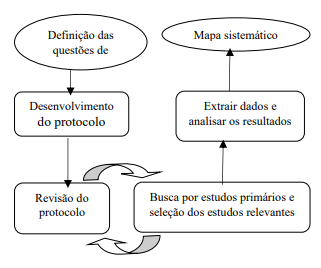
\includegraphics[scale=1.0]{Imagens/mapeamento.png} 
  
  \legend{Fonte: Adaptado de \cite{kitchenham2004procedures}
  }
  \label{fig:fig0}
\end{figure}

\subsection{Planejamento da revisão}

Nesta primeira fase de planejamento, será informado o propósito e os objetivos do
trabalho; as fontes, estratégias e questões de pesquisa; os critérios e procedimentos de seleção
dos resultados; e a forma de extração dos dados destes resultados.

\subsubsection{Questões de pesquisa}
Segundo \cite{kitchenham2004procedures}, formular as questões de pesquisa é a atividade de maior importância ao realizar uma revisão sistemática. Além disso,
as questões de pesquisa visam descobrir tendências de pesquisa (p.ex., tendência de publicação ao longo do tempo, tópicos cobertos na literatura etc.) \cite{Kraemer:2007:HFS:1289816.1289837,kitchenham2004procedures,petersen2008systematic}. Dessa forma, as seguintes questões de pesquisa foram estabelidas:


\begin{enumerate}
     \item[Q1.] Quais frameworks são usadas atualmente desenvolver chatbots ?
    \item[Q2.] Quantas Frameworks são open source ?
    \item[Q3.] Qual o custo de utilização dessas frameworks ?
    \item[Q4.] Quais frameworks realizam processamento de linguagem natural ?
    \item[Q5.] Quais são as características destas frameworks ?
\end{enumerate}

\subsubsection{Estratégias de busca }
Esta seção descreve as fontes de pesquisa e como foram realizadas as buscas, bem como as palavras-chave
que geraram a string de busca e as línguas aceitas para os resultados selecionados.

Foram selecionadas cinco bases bibliográficas, nas quais foi realizada a busca por estes
trabalhos, esta atividade foi realizada no mês de janeiro de 2019 e os resultados retornados
correspondem ao que tinha disponível até esta data.

Para este mapeamento foram utilizadas as seguintes
bases de dados: Scopus, IEEE, science direct, webof science, conpendex e ACM.

\subsubsection{Critérios de Seleção}
De acordo com as questões de pesquisa e com o objetivo da revisão foram definidos
critérios de inclusão e exclusão relevantes para o tema da pesquisa, com o objetivo de nortear a
seleção dos artigos na fase de condução da revisão. Foram elaborados 4 critérios de inclusão (I)
e 4 critérios de exclusão (E) como apresentados abaixo.

Os critérios de inclusão considerados na seleção dos artigos:

\begin{itemize}
    \item I1. O artigo possui informações pertinentes ao escopo do trabalho a exemplo pesquisas de interesse e dados relacionados a frameworks ou plataformas de desenvolvimento de chatbots.
        \item I1. O artigo apresenta alguma ferramenta ou método para desenvolvimento de chatbots.
    
\end{itemize}

Os critérios de exclusão considerados na seleção dos artigos:

\begin{itemize}

    \item E1. No artigo a temática de frameworks para desenvolvimento de chatbots não é abordada.
    \item E2. O artigo apresenta alguma aplicação ou desenvolvimento de chatbots específicos.
    
\end{itemize}

\subsubsection{String de Busca}
Como etapa final do planejamento da revisão foi definida uma string de busca. Para
este fim foram consideradas as palavras chaves do assunto de interesse e seus sinônimos como
apresentados na tabela \ref{tab:termosBusca}.



\begin{table}[H]
    
    \begin{center}
    \begin{tabular}{||c c||} 
    \hline
    Termos & Sinônimos \\ [0.5ex] 
    \hline
    Bot & Chatbot, Chat-bot, Chatterbot   \\ 
    \hline
    Framework & Platform  \\
    \hline
    Development & Building \\
    \hline
    \end{tabular}
    \caption{Termos e sinônimos.}
    \label{tab:termosBusca}
    
    \end{center}
   
\end{table}


Com os termos da pesquisa definidos e utilizando os operadores booleanos <AND> (E) e
<OR> (OU) foi elaborada uma string genérica de busca (Tabela \ref{tab:stringGenerica}), a qual foi utilizada nas bases
bibliográficas durante a seleção dos artigos.

\begin{table}[H]
    
    \begin{center}
    \begin{tabular}{| c |} 
    \hline
    (bot OR chatbot OR chat-bot OR chatterbots) AND (building platform OR development framework) \\ 
    \hline
    \end{tabular}
    \caption{String genérica de busca.}
    \label{tab:stringGenerica}
    
    \end{center}
   
\end{table}


\subsection{Seleção dos estudos primários}

Utilizando a string genérica e alguns filtros nas diferentes bases, foram coletados os
artigos de interesse para o trabalho. Determinou-se um período limite em algumas bases para
refinar os resultados de forma que fossem retornados os artigos mais recentes, para isso foi
definido um filtro de data a partir de anos maiores que 2015 para a Science Direct, de 2000 a
2018 para a IEEE e Scopus, e por fim 2014 a 2019 para a Web of Science.
As strings geradas em cada base de acordo com as entradas utilizadas são as especificadas na
tabela \ref{tab:stringBase}.


\begin{table}[H]
    
    \begin{center}
    \begin{tabular}{| p{5cm}| p{10cm}|}
    \hline
     Base & String\\
    \hline
     Science direct & (chatbot OR chatterbots) AND (development framework)
Filters Applied: 2015-2019 \\ 
    \hline
     IEEE & (bot OR chatbot OR chat-bot OR chatterbots) AND (building platform OR development framework)
Filters Applied: 2000-2018\\ 
    \hline
     Scopus & (bot OR chatbot OR chat-bot OR chatterbots) AND (building platform OR development framework)Filters Applied: nenhum mas trouxe resultados entre 2002-2018\\ 
    \hline
     Web of science & (bot OR chatbot OR chat-bot OR chatterbots) AND (building platform OR development framework) Filters Applied: Últimos 5 anos. Índices: SCI-EXPANDED, SSCI, A\&HCI, CPCI-S, CPCI-SSH, ESCI.\\
     \hline
    \end{tabular}
    \caption{ String de busca de cada base.}
    \label{tab:stringBase}
    
    \end{center}
   
\end{table}

Dessa forma a distribuição de artigos por base ficou como apresentado na figura \ref{fig:bases}, sendo
a IEEE com 58 artigos, a base com o maior número de resultados, seguido da
Science direct com 57, Web of science com 48 artigos, por fim com o menor
número de resultados o Scopus com 13 artigos.


\begin{figure}[H]
  \caption{Quantidade de Artigos coletados por base}

  \centering
  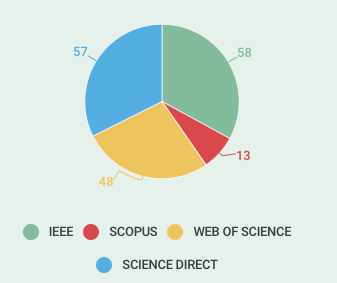
\includegraphics[scale=0.8]{Imagens/grafico_bases.png} 

  \label{fig:bases}
  Fonte: O autor
\end{figure}

O processo de seleção se caracterizou em etapas. Inicialmente foram baixados os arquivos
bibtex de todos os artigos retornados pelas bases através da \textit{string} de busca inserida, para então começar o
processo de seleção. 

No processo de seleção foram lidos os títulos, resumos e palavras-chave para então serem
escolhidos os artigos que foram relevantes de acordo com os critérios. Uma vez que esta pré-seleção foi realizada, foram separados 12 artigos para serem analisados mais
profundamente, explorando mais do seu conteúdo.

Após a leitura dos 12 artigos selecionados para extração de características foi constatado que nenhum atendia as características desejadas, já que não tratavam de \textit{frameworks} para desenvolvimento, mas soluções específicas de \textit{chatbots} ou algoritmos. Esse resultado sugere que esse tipo \textit{framework} não é um tema abordado e publicado nas bases pesquisadas.


\section{ Revisão de Produtos do Mercado}
Não apenas os artigos foram analisados, como também as ferramentas existentes no
mercado para desenvolvimento de chatbots. Um processo de seleção semelhante ao dos
artigos aconteceu na Revisão de Produtos no Mercado, na qual a partir de diferentes strings de
busca inseridas na ferramenta de pesquisa da Google uma lista de frameworks foi
selecionada. Das 33 frameworks que foram retornados nas buscas, 14 open source foram escolhidos para uma
análise mais aprofundada e por fim 4 foram tomados como referência para o produto de software
desenvolvido neste trabalho.


Uma pesquisa na plataforma stack overflow\footnote{O Stackoverflow é um website de perguntas e respostas, criado em 2008, mundialmente usado por desenvolvedores, engenheiros de software e pesquisadores para compartilhar conhecimento e sanar dúvidas relacionadas a tecnologia e outras áreas. Website: https://stackoverflow.com} foi realizada estabelecer um indicativo de que tais frameworks ou plataformas estão em uso na comunidade de desenvolvedores e no mercado. A figura \ref{fig:frameworks} representa a quantidade de perguntas relacionadas a cada framework.


\begin{figure}[H]
  \caption{Quantidade de perguntas em cada framework no stackoverflow}

  \centering
  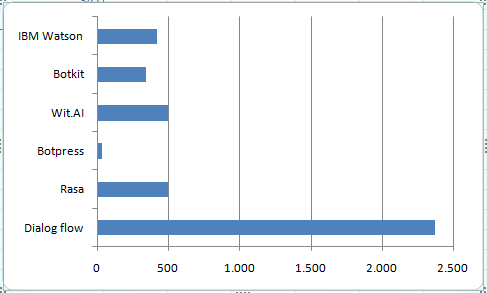
\includegraphics[scale=1]{Imagens/frameworks-stack.png} 

  \label{fig:frameworks}
  Fonte: O autor
\end{figure}

Devido a alta popularidade, o IBM Watson Assistant e Dialog Flow foram selecionados para uma comparação apesar de não serem open source. Vale ressaltar que o Botpress e IBM Watson possuem suas próprias áreas de perguntas onde a comunidade de desenvolvedores interage. 


\begin{itemize}
    \item Botpres \footnote{Fórum em :https://help.botpress.io/top}: 383 perguntas
    \item IBM Watson Assistant \footnote{Fórum em: https://developer.ibm.com/answers/smartspace/watson/index.html}: 4063 perguntas 
\end{itemize}



O Quadro apresenta as frameworks analisados e os URls para acesso a estas. Além disso, responde a primeira questão de pesquisa.

Quais frameworks open source são usadas atualmente desenvolver chatbots ?


\begin{table}[H]
    
    \begin{center}
    \begin{tabular}{| p{3cm}| p{3cm}|  p{3cm}|}
    \hline
     Framework & URL & Licensa\\
    \hline
    Rasa & https://rasa.com/ & Apache 2.0 \\
    \hline
    Wit.ai & https://wit.ai/ & MIT License \\
    \hline
    Botpress & https://botpress.io/ &  AGPLv3 e Licensa proprietária Botpress \\
    \hline
    Botkit & https://botkit.ai/ & MIT license \\
    \hline
    
    \end{tabular}
    \caption{ Frameworks e respectivas urls e licensas}
    
    \end{center}
   
\end{table}

As seções seguintes descrevem o que foi encontrado na exploração destas frameworks, apresentando como cada uma delas funciona.


\subsection{Rasa}

A framework Rasa ou Rasa Stack possui um conjunto de ferramentas de aprendizado de máquina para que desenvolvedores possam criar chatbots contextuais, diferente de daqueles baseados em regras pré-definidas. Essa framework é composta de dois módulos que são independentes e podem ser usados separadamente. O módulo principal (Rasa Core) e módulo de processamento de linguagem natural (chamado de Rasa natural language understanding ou Rasa NLU) são detalhados a seguir:

\begin{enumerate}
    \item Rasa Core (Núcleo): È uma ferramenta que usa aprendizado de máquina para inferir possíveis ações a serem executadas pelo chatbot. O aprendizado de máquina é feito com o constante feedback do usuário, e a partir disso, são calculadas as probabilidades de execução de cada ação. Essa abordagem é conhecida como aprendizado iterativo.
    \item Rasa NLU: È uma ferramenta para processamento de linguaguem natural open source capaz de classificar intenções dos usuários e extrair entidadades em chatbots. Sendo assim, é possível extrair dados estruturados de uma conversa em linguagem natural. Vale ressaltar que esse módulo pode ser executado em qualquer ambiente sem depender de chamadas á api's externas como as do Google, IBM Watson ou Microsoft.
    
\end{enumerate}

A integração com canais de comunicação nessa framework é possível de forma programática nos seguintes canais:

\begin{itemize}
    \item Web
    \item Facebook Messenger
    \item Slack
    \item Twilio
    \item Google Hangouts\footnote{https://hangouts.google.com}
    \item Microsoft Teams\footnote{https://products.office.com/pt-br/microsoft-teams}
    \item Webex Teams\footnote{https://www.webex.com}
    \item Conectores customizados
\end{itemize}



\subsection{Wit.ai}

Wit.ai é uma plataforma que implementa uma API (do inglês application program interface) gratuita para instancias públicas e privadas sem limitações para requisições. Fornece reconhecimento de voz e texto por meio do apredizado de máquina. Além disso, possui elementos como a classificação de intenções e extração de entidades. Também disponibiliza entidades pré-definidas como temperaturas, números, email e outras entidades comumente utilizadas em chatbots.

Essa plataforma foi adquirida pelo facebook em 2015 e, portanto, pode ser integrado com mais facilidade com o facebook messenger. O algoritmo de apredizado dessa plataforma é baseado em histórias (casos de uso dependentes de domínio). Além disso, Essa plataforma possui inteface de programação gráfica, possibilitando assim que usuários sem conhecimento de programação possam desenvolver chatbots. 

A desvantagem do Wit.ai é o fato ser uma solução hospedada pelo facebook onde os recursos são centralizados e somente disponíveis via requisições http. Além do mais, só permite integração com o Facebook Messenger.


\subsection{Botpres}
Botpres é uma framework que possibilita a integração com as principais plataformas de mensagens como Telegram, facebook messenger, slack e etc. A arquitetura dessa framework é modular, ou seja, permite a integração com módulos internos, externos, ou módulos criados e personalizados pelo desenvolvedor. A proposta da framework é fornecer um ambiente para a criação de novos módulos que podem ser integrados como plugins wordpress \footnote{WordPress é um sistema livre e aberto de gestão de conteúdo para internet, baseado em PHP com banco de dados MySQL, executado em um servidor interpretador, voltado principalmente para a criação de páginas eletrônicas e blogs online.} (De fato, o wordpress para chatbots).

Outras funcionalidades são gerenciamento do fluxo conversacional via interface, suporte ao processamento de várias linguagens, ferramenta para análise estatísticas e a possibilidade de intervenção humana quando o chatbot não consegue resolver ou entender algum problema. Além disso, possui uma estrutura que facilita a integração nos seguintes canais:

\begin{itemize}
    \item Web
    \item Facebook Messenger
    \item Slack
    \item Microsoft Teams\footnote{https://products.office.com/pt-br/microsoft-teams}
\end{itemize}

\subsubsection{Tabela de preços}

Apesar de ser \textit{open source}, a proposta do Botpress atualmente é que somente grandes empresas serão cobradas pelo uso da \textit{framework}. No futuro serviços e ferramentas \textit{premium} também serão ofertadas e cobradas. A figura \ref{fig:bot-planos} apresenta os planos.

\begin{figure}[H]
  \caption{Planos da framework botpress}

  \centering
  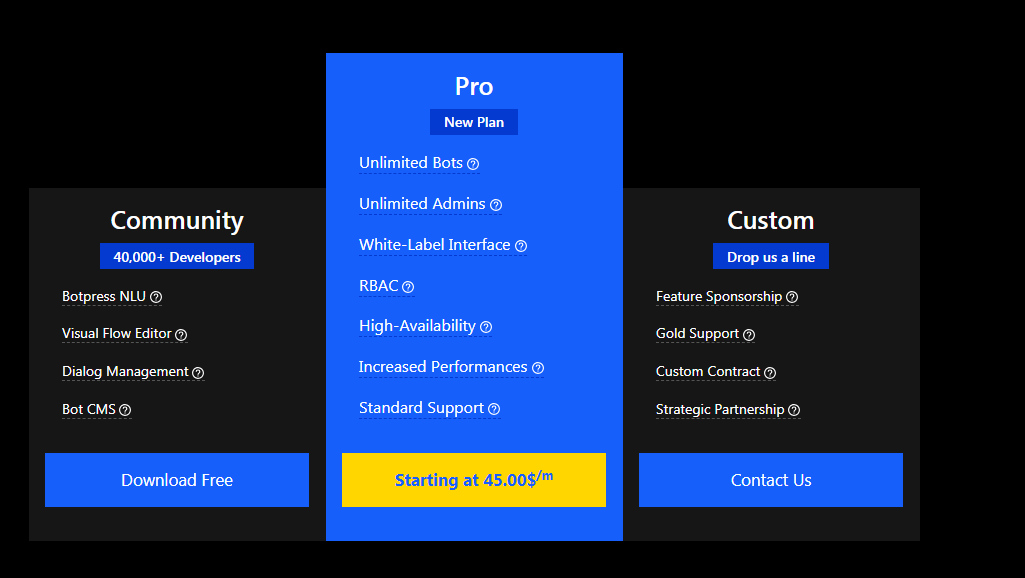
\includegraphics[scale=0.5]{Imagens/botpress-precos.png} 
 
  \label{fig:bot-planos}
  Fonte: https://botpress.io/pricing
\end{figure}



\subsection{Botkit}

É uma framework open source que foi adquidira pela Microsoft em novembro de 2018. Essa framework disponibiliza nativamente funcões de desenvolvimento de chatbots simples e baseados em regras. Entrentanto, a principal vantagem é a flexibilidade de utilizar essa framework em conjunto com outras que possuem métodos de processamento de linguagem natural para atribuir maior inteligencia ao conversador. Além disso, possui uma estrutura que facilita a integração nos seguintes canais:

\begin{itemize}
    \item Web
    \item Facebook Messenger
    \item Slack
    \item Twilio
    \item Google Hangouts\footnote{https://hangouts.google.com}
    \item Microsoft Teams\footnote{https://products.office.com/pt-br/microsoft-teams}
    \item Webex Teams\footnote{https://www.webex.com}
\end{itemize}


Devido a aquisição da framework pela Microsoft o site oficial recomenda a utilização do botkit com ferramentas de processamento de linguagem natural  da empresa, Luis.ai. Além disso,  a integração de um chatbot construido com o botkit em outros canais de comunicação como Telegram e whatsapp é recomendada utiliazando o Microsoft Bot Framework\footnote{https://dev.botframework.com/} onde também é possível realizar análise estatísticas das conversas realizadas no chatbot. O uso dos recursos essa framework Microsoft é pago, porém é possivel utilizar somente o botkit de forma independente.

\subsection{IBM Watson}

O IBM Watson é uma plataforma que oferece serviços de computação cognitiva. A IBM lançou a plataforma em 2011 e o nome é em homenagem ao  CEO Thomas J. Watson.

A computação cognitiva é uma mistura de diversas técnicas como processamento de linguagem natural, aprendizado de máquina, inteligencia artificial e etc. Também possui serviços como reconhecimento e análise de vídeos e imagem; interação por voz; leitura de grandes volumes de textos.

O IBM Watson é uma plataforma que oferece outros serviços na nuvem, entretanto, para o desenvolvimento de chatbots é utilizado o Watson Assistent.

As características do Watson Assistent são:


\begin{itemize}
    \item Conteúdo pré-construído: Adicione atendimento ao cliente e outros pacotes específicos de cada área (finança, saúde, etc) prontos para iniciar seu assistente.
    \item Desambiguação: Quando uma requisição do usuário não está clara, o Watson irá automaticamente propor múltiplos opções em vez de responder incorretamente.
    \item Resolução de conflitos de Intenção:
Uso de inteligência artificial para identificar erros introduzidos por humanos nos dados de treinamento.
    \item Recomendação de Intenção: Uso dos dados de conversas existentes para treinar o assistente mais rápido.
    \item Habilidade de Busca: Realiza busca em dados desestruturados para ampliar o conhecimento do assistente
    
    \item Linguagem natural: Processa linguagem natural e realiza conversão tanto de voz para texto quanto de texto para voz.

\end{itemize}


A possibilidade de integração em diversos canais é facilitada por essas plataforma pois essa funcionalidade é entregada ao desenvolvedor a partir do preenchimento de alguns formulários simples com informações sobre o canal. Alias um grande diferencial é que além dos canais convencionais é feita integração com dispositivos IOT\footnote{Internet das coisas, em inglês Internet of Things (IOT)}.


\subsubsection{Tabela de Preços}

Os custos relacionados ao uso da plataforma dependem do plano e recursos demandados. Existe um plano gratuido que dura um mês para testar a plataforma e após esse período precisa ser migrado para algum dos outros planos pagos. As figuras \ref{fig:basico} e \ref{fig:avancado} apresentam mais detalhes sobre os planos. 



\begin{figure}[H]
  \caption{Planos básicos da plataforma IBM Watson Assistant}

  \centering
  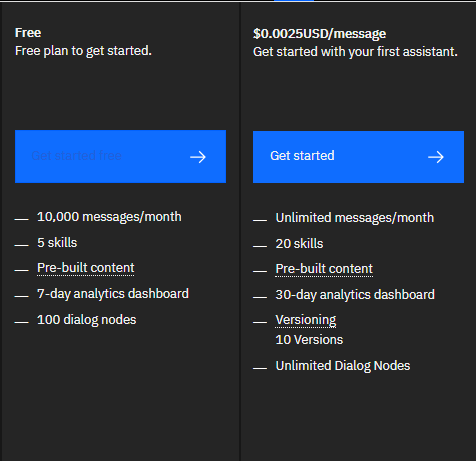
\includegraphics[scale=0.5]{Imagens/ibm-basic.png} 
 
  \label{fig:basico}
  
  Fonte: https://www.ibm.com/cloud/watson-assistant/pricing/
\end{figure}



\begin{figure}[H]
  \caption{Planos avançados da plataforma IBM Watson Assistant}

  \centering
  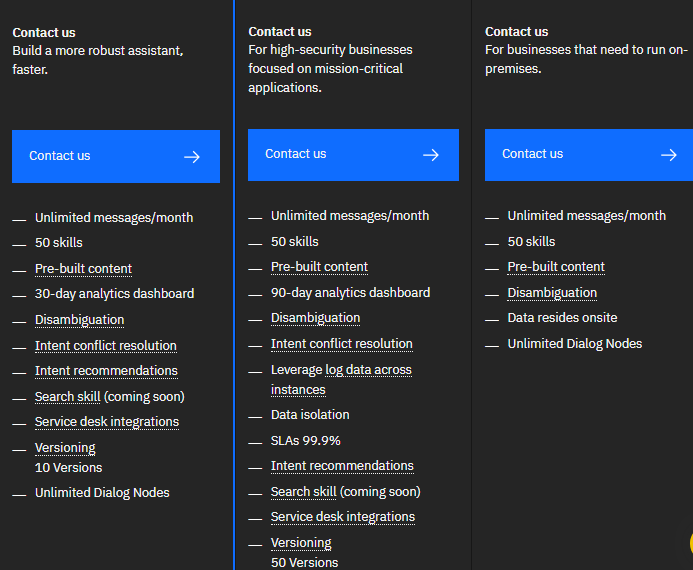
\includegraphics[scale=0.5]{Imagens/ibm-other.png} 
 
  \label{fig:avancado}
    Fonte: https://www.ibm.com/cloud/watson-assistant/pricing/
\end{figure}



Para a maioria das aplicações o plano lite parece ser adequado, entretanto, quando existe a necessidade de utilizar outros recursos é preciso entrar em contato com a IBM para que se possa obter um orçamento dos custos. 

A tabela \ref{tabela:simulacaoIBM} foi elabora para fornecer uma visão geral dos custo associados ao uso da plataforma da IBM.


\begin{table}[H]
    
    \begin{center}
    \begin{tabular}{| p{3cm}| p{3cm} | p{3cm}|}
     \hline
      N° Mensagens & USD & Real\\
    \hline
     2.000 & 5,00 &  18,68 \\
    
    \hline
     5.000 & 12,5 & 45,62  \\
    
    \hline
     10.000 & 25,00 & 93,25 \\
    
    \hline
     30.000 & 75,00 & 279,75\\
    \hline
   
   
    \end{tabular}
    \caption{Simulação de preços baseada no plano Lite do IBM Watson Assistant}
    \label{tabela:simulacaoIBM}
    \end{center}
   
\end{table}


\subsection{Dialog Flow}

Dialog Flow é uma plataforma do google, antes chamada de API.AI, que fornece ferramentas para processamento de conversas em linguagem natural. 

A principais características dessas plataforma são :

\begin{itemize}
    \item Processamento de Linguagem Natural: Processamento de dados em linguagem natural e classificação de intenção e entidades
    \item Aprendizado de máquina: Uso de dados para treinamento e melhora da interação aplicada ao domínio do problema
    \item Contexto: Controle do estado atual, ou dados , das conversas com os usuários. Esses dados podem ser usados como input ou output para eventos ou qualquer eventual processamento.
    \item Pode ser integrado com qualquer plataforma de mensageiros como Facebok, slack etc. Além de ser integrável com dispositivos móveis e weareables.
    \item Análise estatística dos dados 
\end{itemize}

Além disso, uma vantagem distinta do Dialogflow é o seu programa de análise, chamado de chatbase. O Google já é um elemento importante da análise da web e de usuários, graças à sua plataforma do Google Analytics \footnote{https://analytics.google.com/analytics/} estabelecida há muito tempo. 

 As integrações em um clique no Dialogflow, é possível gerenciar a integração do agente com o Google Assistente por meio do Actions on Google e muitas outras plataformas de mensagens famosas, como o Slack, o Facebook Messenger e o Twitter. Além disso, o Dialogflow facilita a exportação ou importação de agentes de/para outras plataformas de processamento de linguagem natural, como o Amazon Alexa e o Microsoft Cortana.


\subsubsection{Tabela de preços}

O Dialog Flow possui um plano gratuito porém com funções limitadas e outro pago para empresas. Os preços e características de cada plano são apresentados na figura \ref{fig:dialog-precos}.



\begin{figure}[H]
  \caption{Planos da plataforma Dialog Flow}

  \centering
  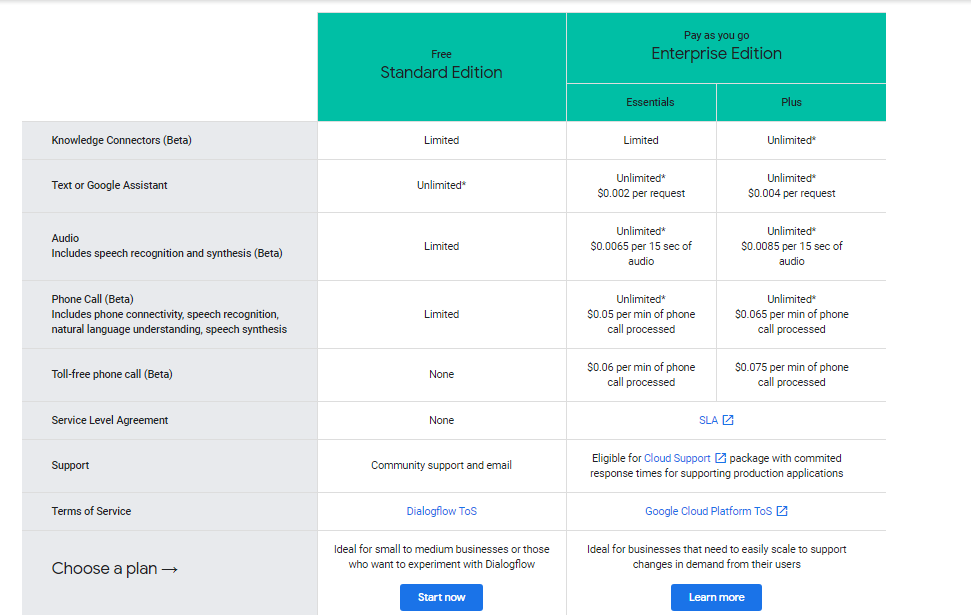
\includegraphics[scale=0.5]{Imagens/dialog-precos.png} 
 
  \label{fig:dialog-precos}
  
  Fonte: https://cloud.google.com/dialogflow/pricing
\end{figure}




\subsection{Extração de características}

A partir da exploração dos 4 aplicativos 7 características foram extraídas. As principais características encontradas nas frameworks estão discriminadas no Quadro \ref{tabela:caracteristicas}, assim como suas respectivas identificações.

\begin{table}[H]
    
    \begin{center}
    \begin{tabular}{| p{5cm}| p{5cm}|}
    \hline
     Identificação & Características\\
    \hline
    C1 & Open source\\
    \hline
    C2 & Integração com mensageiros externos \\
    \hline
    C3 &  Processa linguagem natural\\
    \hline
    C4 & Usa aprendizado de maquina para inferir contexto \\
    \hline
    C5 & Processa áudio \\
    \hline
    C6 & Fornece interface  gráfica \\
    \hline
    C7 & Realiza análise estatística \\
    \hline
   
    \end{tabular}
    \caption{ Principais características identificadas nas frameworks}
    \label{tabela:caracteristicas}
    \end{center}
   
\end{table}

A partir do levantamento destas características foi construído um quadro associando estas a cada uma das frameworks. O Quadro \ref{tabela:comparativo} exibe quais característica são apresentadas por cada framework, respondendo assim, a segunda e terceira questão de pesquisa.

Quais frameworks realizam processamento de linguagem natural ?

Quais são as características destas frameworks?


\begin{table}[H]
    
    \begin{center}
    \begin{tabular}{| p{2cm}| p{1cm}| p{1cm} | p{1cm}| p{1cm}| p{1cm}| p{1cm}| p{1cm}|}
     \hline
       & C1 & C2 & C3 & C4 & C5 & C6 & C7\\
    \hline
     Dialog Flow &  &   & X & X & X  &  &  \\
     \hline
     Watson Assistant &  &   & X & X &   &  &  \\
    
    \hline
     Rasa & X &   & X & X &   &  &  \\
    
    \hline
     Wit.ai & X &   & X & X & X &  &  \\
    
    \hline
     Botpress & X & X & X &  &   & X & X\\
    
    \hline
     Botkit & X & X &   &   & X & X & X\\
    
   \hline
   
    \end{tabular}
    \caption{ Principais características identificadas nas frameworks}
    \label{tabela:comparativo}
    \end{center}
   
\end{table}


\subsection{Escolha das Frameworks}


Decidir qual framework será mais adequada para um projeto de software não é tarefa trivial. Em seu famoso artigo \textit{“No Silver Bullet — Essence and Accident in Software Engineering"} (Não há bala de prata — Essência e Acidente na Engenharia de Software em português), Frederick P. Brooks afirmou, em 1986, que não existe nenhuma metodologia de desenvolvimento ou técnicas de gestão que consiga aumentar significativamente a produtividade e confiabilidade da engenharia de software. Assim, de forma analoga, não existe a framework perfeita e, portanto, a escolha da mesma deve levar em conta os requisitos e restrições do projeto em questão.

Sendo assim, os requisitos gerais e suficientemente amplos de forma que sirvam de referência para este trabalho e projetos futuros. Esse requisitos gerais também podem ser entendidos como recursos ou habilidades que um chatbot necessita e que a framework escolhida deve prover. Também é possivel que se utilize mais de uma framework para atender os requisitos do projeto.


\begin{itemize}
    \item \textbf{NLP: } O chatbot deve ter um módulo de processamento de linguagem natural
    \item\textbf{ IA:}  O chatbot deve possuir algoritmos de aprendizado de máquina para que possa entender contextos de conversação e ampliar sua base de conhecimento.
    \item \textbf{Canais: } O chatbot deve estar presente em mais de um canal de comunicação
    \item\textbf{ Hospedagem:}  O chatbot não deve depender de um serviço de hospedagem específico podendo ser hospedado em qualquer infraestrutura disponível e de acordo com as restrições orçamentárias do projeto. 
    
\end{itemize}

Vale ressaltar que um outro critério importante a se considerar na escolha da framework é o tamanho da comunidade que a mantém atualizada e realiza correções frequentes. Nesse ponto, todas as frameworks selecionadas na fase de levantamento possuem comunidade ativa.  

A partir dos critérios selecionados as frameworks Botkit e Rasa foram selecionadas. O diagrama da figura \ref{fig:frame-decisao} ilustra o processo de tomada de decisão.

\begin{figure}[H]
  \caption{Diagrama ilustrativo do processo de escolha das frameworks de desenvolvimento.}

  \centering
  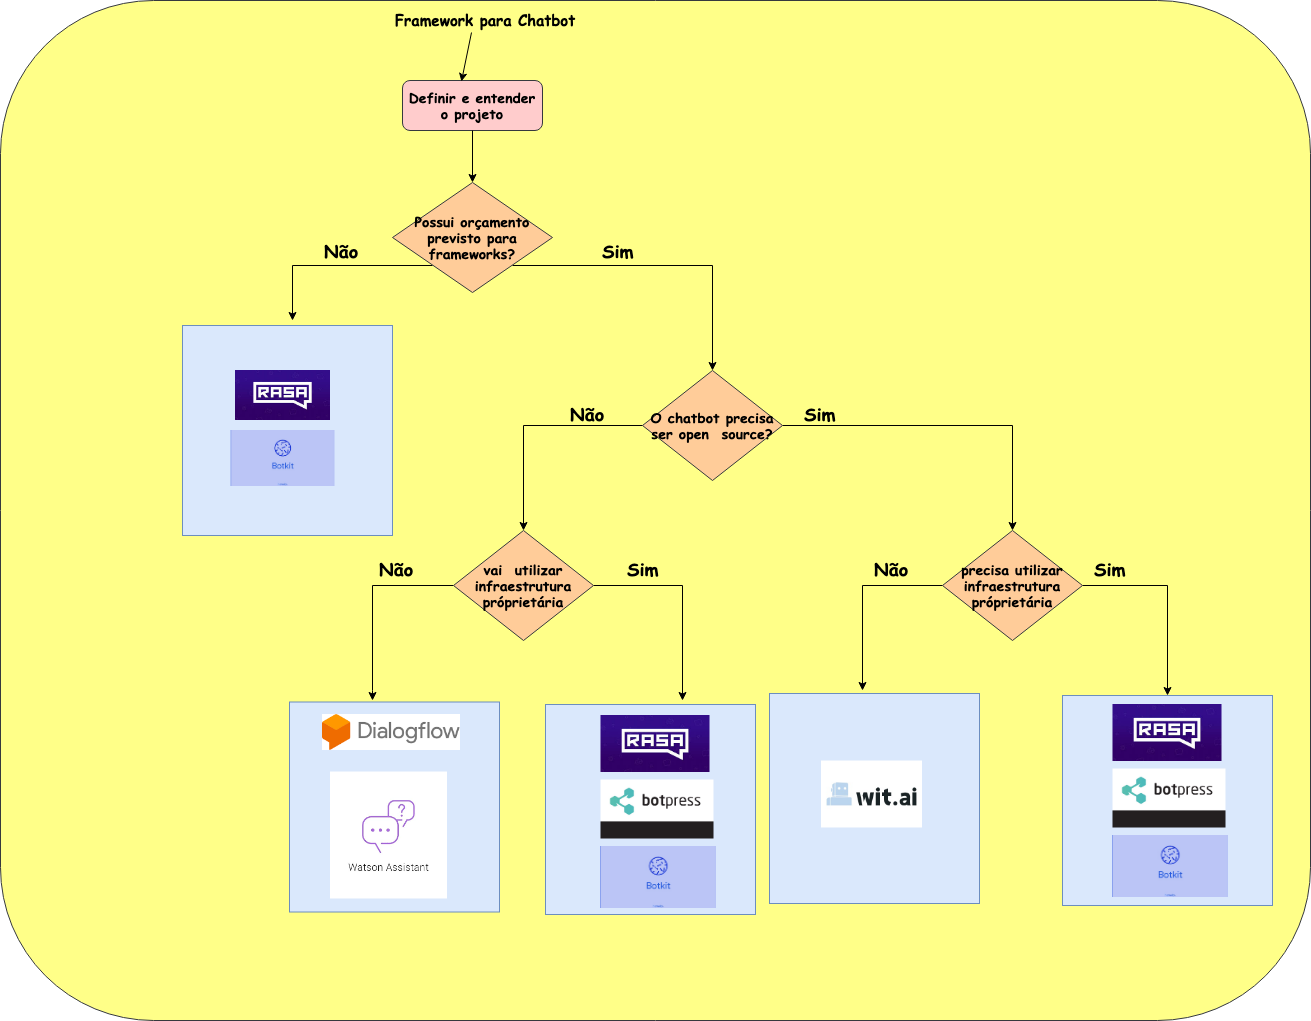
\includegraphics[scale=0.37]{Imagens/decisao_frame.png} 
  \label{fig:frame-decisao}
  Fonte: O autor.
\end{figure}



As frameworks Botkit e Rasa com o objetivo de abranger todas as 7 características definidas. Essas frameworks permitem que as soluções desenvolvidas sejam escaláveis, uma vez que fornece total domínio dos dados e do código interno, são independentes de infraestrutura e permitem integração em múltiplos canais. 

As frameworks Dialog Flow, IBM Watson Assistant e Wit.ai são altamente dependentes de serviços hospedados em servidores proprietários. Portanto, possuem limitações em termos custos, domínio dos dados de aplicações e escalabilidade. 







\chapter{Desenvolvimento}
Nesta seção serão explicados os passos utilizados no desenvolvimento da interface de integração de chatbots em mais de um canal de comunicação. Os canais propostos inicialmente foram uma pagina web e o Slack. Além disso, O WhatsApp foi usando como canal complementar aos objetivos iniciais e forma de avaliar a dificuldade e o aspectos relacionados a possibilidade de estender o número de canais de comunicação.



\section{Desenvolvimento da Arquitetura}

Foi desenvolvido um chatbot composto por três componentes principais: Uma ou mais interface de comunicação com o usuário final (como Slack e paginas web), um componente de processamento de linguagem natural e um servidor webhook para gerenciar a troca de mensagens. 

Para processamento de linguagem natural foi utilizada a framework Rasa para mapear texto natural em dados estruturados como intenções e entidades bem como guiar o fluxo da conversa. O chatbot utilizado para integração possui um diálogo simples que busca identificar se um cliente em potencial possui interesse na compra e venda de determinados imóveis. Vale ressaltar que o  domínio em que se encontra o chatbot está fora do escopo deste trabalho.

\subsection{Webhooks}
Para que seja possível a integração de um agente conversacional, chatbot, em mais de um canal de comunicação é preciso que exista uma serviço que realize o gerenciamento das conversas e possa distribui-las em diferentes interfaces.

Webhooks, segundo a \citeonline{sendgrid2014webhook}, são uma forma de recebimento de informações, baseada em eventos, entre dois ou mais sistemas. Também chamado de \textit{Web callback}, em referência a funções ou rotinas que são executadas quando determinados eventos acontecem. Em suma,  webhooks são funções ou rotinas que são executadas quando notificadas da ocorrência de determinados eventos via HTTP (HyperText Transfer Protocol que em português significa Protocolo de Transferência de Hipertexto). Dessa forma, uma ação executada em um sistema A dispara uma ação em um sistema B.

O webhook também é chamado de API (Application Programming Interface que em português significa Interface de Programação de Aplicativos) reversa. Vale ressaltar que ambas abordagens possuem fatores comuns como o uso do protocolo HTTP e a implementação de funções ou rotinas definidas pelo usuário. A diferença é:

    \begin{itemize}
        \item Um webhook é baseado em eventos, ou seja, dois sistemas trocam informações e executam ações somente quando determinadas eventos acontecem.
        \item Uma API é guiada por requisições HTTP e, portanto, para um sistema A descobrir se determinado evento ocorreu em um sistema B precisaria realizar requisições frequentes para assim descobrir sobre o estado atual sistema B.  
    \end{itemize}

A figura \ref{fig:webhookdiff} ilustra a diferença fundamental entre as duas abordagens.

\begin{figure}[H]
  \centering
  \caption{Webhook X API ao longo do tempo.}
  \centering
  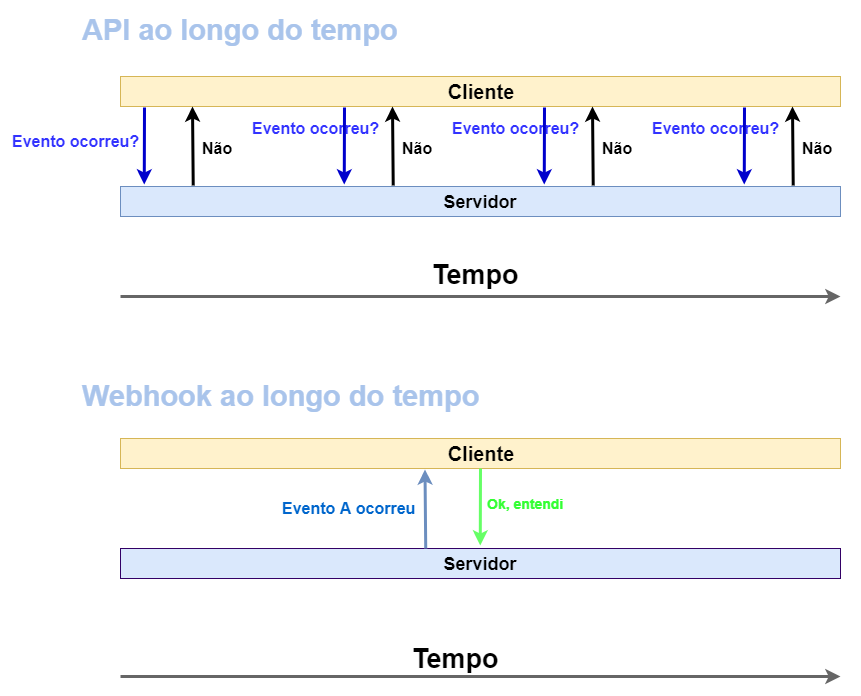
\includegraphics[scale=0.5]{Imagens/webhook-api.png} 
  \label{fig:webhookdiff}
  Fonte: O autor
\end{figure}



\textit{Webhooks}, são capazes de receber informações de sistemas externos sem uso desnecessário da rede e, portanto, foram utilizados para troca de mensagens entre os diferentes canais de comunicação. Assim, para desenvolver aplicações para Slack, Telegram,  Facebook Messenger e outros mensageiros é necessário a implementação de um servidor\textit{ webhook} que esteja esperando por eventos que são enviados pelos mensageiros para comunicação com cada plataforma. Na arquitetura proposta foi desenvolvido um único\textit{ webhook} que implementa a interface de API necessária para que o Slack, uma pagina web e o Whatsapp por meio do Twilio ser integrados com um chatbot.

Para a implementação do webhook foi necessário utilizar a documentação oficial da API do Slack e Twilio\footnote{https://www.twilio.com/} para estabelecer o padrão que deve ser esperado pelo webhook. Assim, Foi implementado um webhook capaz de comunicar-se com o Slack, uma página web e o Whatsapp. O Twilio é uma plataforma na nuvem que fornece chamadas telefônicas e mensagens de texto usando os webhooks e foi usado como um canal adicional neste trabalho.

Foi desenvolvido um servidor utilizando a \textit{framework Botkit} com um \textit{webhook} como interface de comunicação e um \textit{middleware} que realiza requisições (via protocolo http) para uma API de processamento de linguagem natural desenvolvida na framework Rasa. O conceito de middleware é utilizado na framework Botkit referenciando a funções que podem extender e personalizar funcionalidades padrão da framework. De acordo com a documentação oficial qualquer desenvolvedor pode criar seus próprios middlewares para modificar o comportamento da forma mais adequada ao projeto.

A partir disso, a arquitetura do chatbot foi elaborada levando em consideração um princípio da engenharia de software, a separação de interesses. A separação de interesses, de acordo com \citeonline{hursch1995separation} permite a localização de diferentes tipos de informações nos programas, facilitando o desenvolvimento, compreensão, reutilização e modificação. Para isso, cada componente, módulo ou camada do software deve ter uma função concisa cujo comportamento esperado, dado entrada e saída, é conhecido mas sua implementação não deve ser vista por componentes externos. A arquitetura proposta é ilustrada na figura \ref{fig:arquitetura} e o código principal que utiliza o middleware que se comunica com o módulo de processamento de linguaguem natural é apresentado na figura \ref{middleware-rasa}. 


\begin{figure}[H]
  \centering
   \caption{Arquitetura da framework de integração em multiplos canais}
  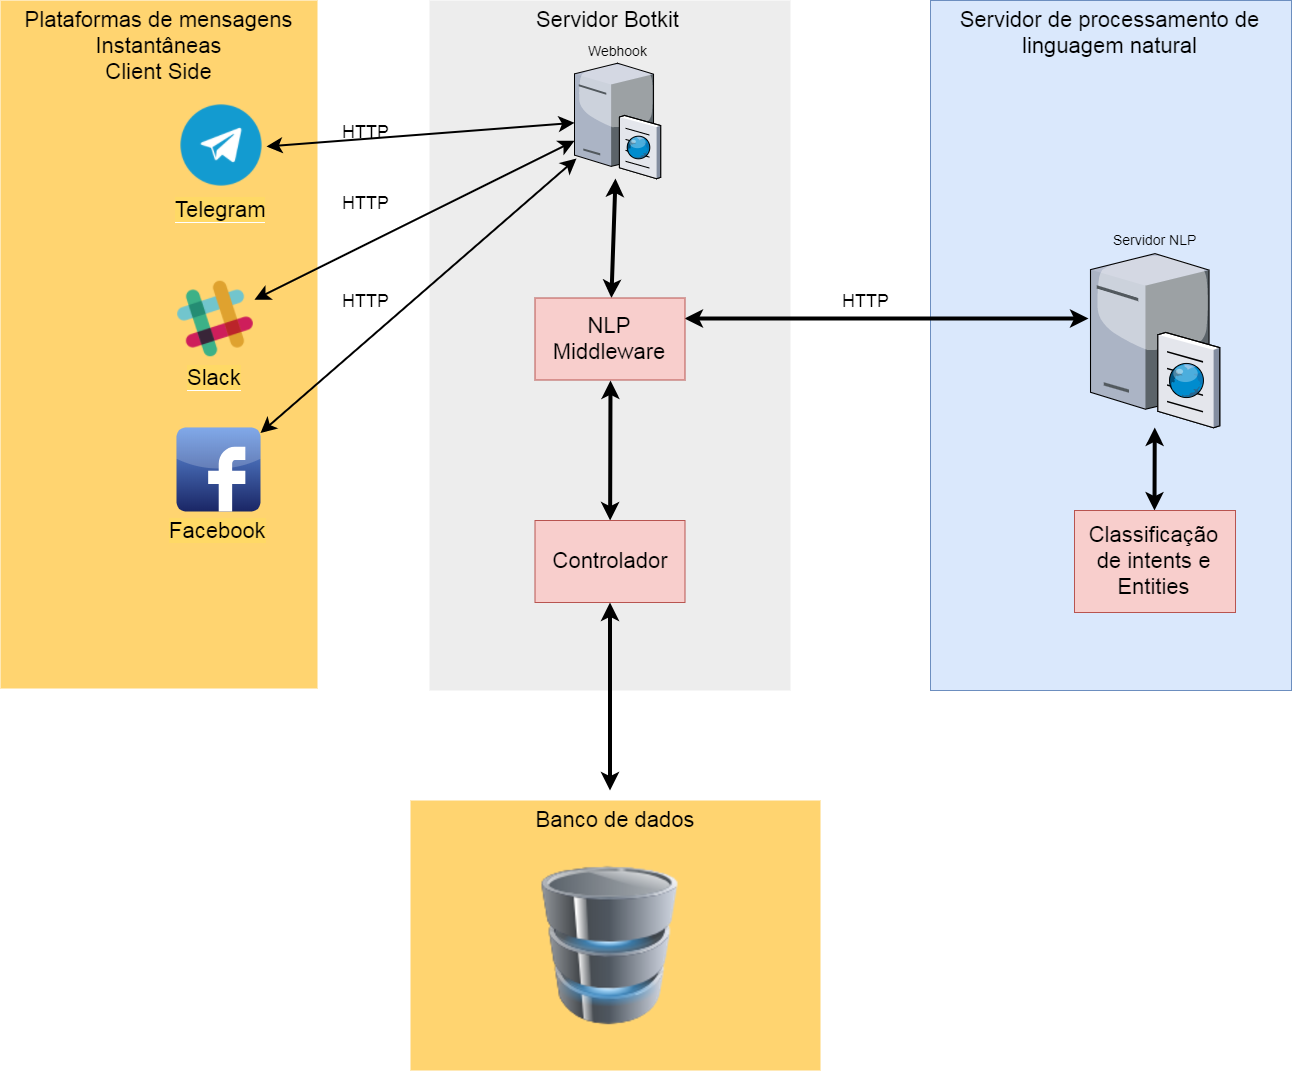
\includegraphics[scale=0.35]{Imagens/Botkit-architecture.png} 
  \label{fig:arquitetura}
  Fonte: O autor.
\end{figure}



\begin{figure}[H]
  \centering
   \caption{Código que utiliza o middleware NLP.}
  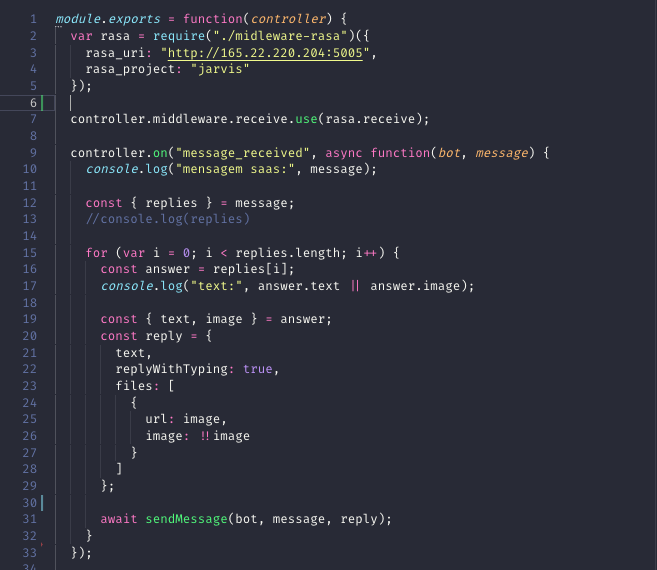
\includegraphics[scale=0.35]{Imagens/nlu-middleware.png} 
  \label{middleware-rasa}
  
\end{figure}


\subsection{Suporte ao protocolo HTTPS}

De acordo com \citeonline{naylor2014cost} o HTTPS é uma extensão segura do protocolo HTTP que utiliza uma camada de criptografia SSL/TLS, em inglês Secure Sockets Layer e Transport Layer Security, para estabelecer uma comunicação segura com o servidor. O SSL/TLS é essencial sempre que houver informações sensíveis sendo transmitidas, como nomes de usuário, senhas e informações de pagamento. 

Como webhooks são basicamente servidores é possível gerar o certificado junto a uma entidade verificada e garantir a autenticidade e segurança das mensagens que estão sendo trocadas. A integração com o Slack foi feita utilizando HTTPS porém nos outros canais foram utilizados somente HTTP.


\subsection{Implementação do Webhook}

O webhook é o intermediador entre o Slack, a pagina web, o whatsapp  e o chatbot. Sendo assim, ele fica esperando requisições HTTP, mais específicamente requisições feitas com o método POST, vindas dos canais de comunicação. A cada mensagem recebida, ele repassa a mensagem ao chatbot que, por sua vez, realiza determinadas ações e envia mensagens de resposta.

O webhook implementado executa em um servidor NodeJS e o mesmo utiliza uma porta para cada canal de comunicação presente na aplicação. Neste trabalho utilizamos três canais de comunicação, portanto, três portas foram usadas.

\subsubsection{Implementação do Webhook para o Slack}

O cérebro de uma aplicação que utiliza  a framework Botkit é chamado de controller (controlador em português).Um controller é uma interface que independe de plataformas e pode ser usado por desenvolvedores para adicionar recursos e funcionalidades ao chatbot. A figura \ref{fig:webhook_slack} mostra a utilização da instancia de um controller para configurar e gerenciar as requisições que serão recebidas do mensageiro Slack.

\begin{figure}[H]
  \centering
   \caption{Código principal do webhook esperando requisições do slack}
  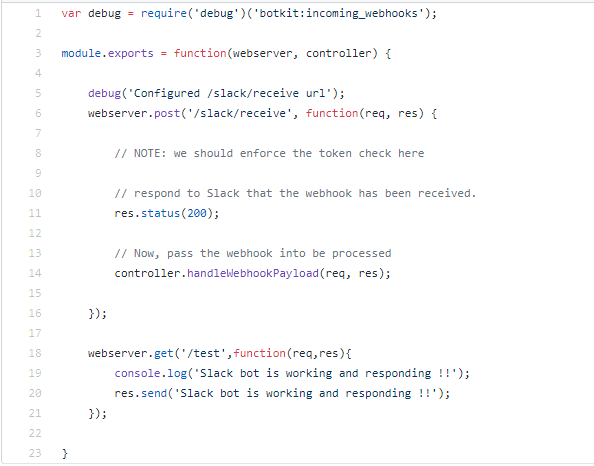
\includegraphics[scale=0.8]{Imagens/webhook_slack.png} 
  \label{fig:webhook_slack}
\end{figure}

\subsubsection{Implementação do Webhook para Web}

A implementação do chatbot na web difere dos mensageiros pois faz-se necessário a implementação de um script, executando no lado do cliente, que seja capaz de enviar requisições para o webhook que está no lado do servidor.

A framework Botkit fornece um script simples, juntamente com um layout html e css, que pode ser executado nos browsers que utiliza a arquitetura cliente-servidor. 

\begin{figure}[H]
  \centering
   \caption{Web Chat do Botkit que executa na arquitetura cliente-servidor  }
  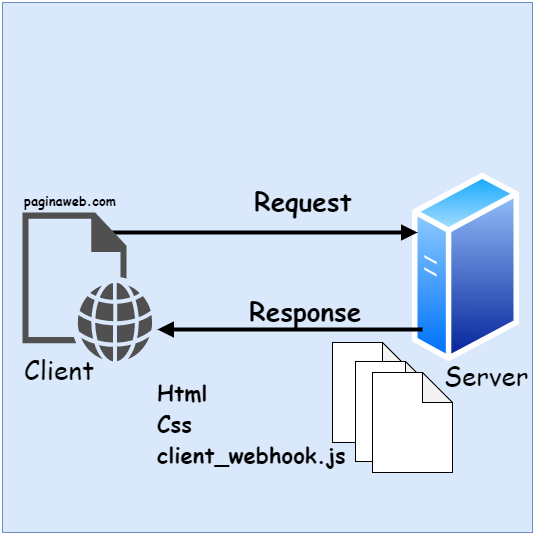
\includegraphics[scale=0.4]{Imagens/http-client.png} 
  \label{fig:http_webhook}
\end{figure}

A figura \ref{fig:http_webhook} mostra como acontece a comunicação cliente-servidor e a renderização da interface do chat juntamento com o script que executa no lado cliente. No Slack, e em outros mensageiros, todos os eventos relacionados a interação entre o usuário e o chatbot são enviados automáticamente para o webhook que definimos.

Na web, o script que executa nos browsers fica aguandando mensagens do usuário e as repassa via http para o webhook do lado do servidor. As figuras \ref{fig:webhook_deliver} e \ref{fig:webhook_code} mostram os códigos responsáveis por essas tarefas. 

\begin{figure}[H]
  \centering
   \caption{Código executado quando o usuário digita uma mensagem}
  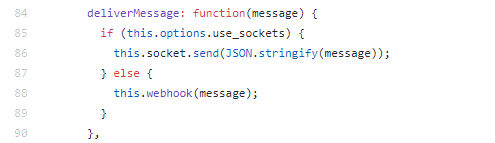
\includegraphics[scale=0.8]{Imagens/deliver_webhook.png} 
  \label{fig:webhook_deliver}
\end{figure}


\begin{figure}[H]
  \centering
   \caption{Código responsável pela comunicação entre cliente-servidor}
  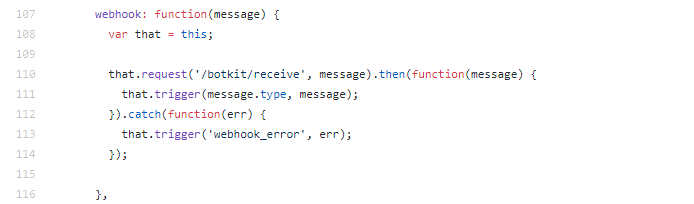
\includegraphics[scale=0.8]{Imagens/webhook_code.png} 
  \label{fig:webhook_code}
\end{figure}


\subsubsection{Formas de utilizar o chatbot na Web}

È importante destacar que a estrutura inicial que o Botkit oferece pode e deve ser customizada para atender aos requisitos do projeto a ser desenvolvido. Além disso, existem três maneira que desenvolvedores podem utilizar o botkit na web:

\begin{itemize}
    \item Iframes com paginas embutidas
    \item Link direto para uma pagina do chatbot
    \item Embutir a interface do chat em uma pagina web existente
\end{itemize}


\begin{figure}[H]
  \centering
   \caption{Código para embutir chatbot em um iframe}
  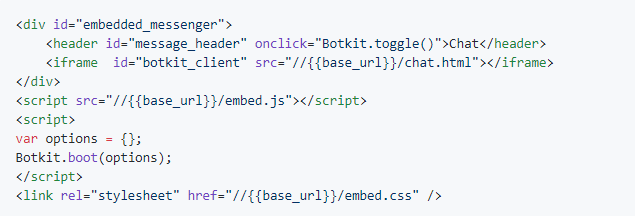
\includegraphics[scale=0.8]{Imagens/iframe.png} 
  \label{iframe}
\end{figure}

O código ilustrado na figura \ref{iframe} é um exemplo de como desenvolvedores podem embutir o chat no lado cliente utilizando a tag iframe do html. Os outros casos de uso requerem habilidades de programação web mas são bem simples.

Em suma, desenvolvedores também podem hospedar diretamente todos os arquivos do chat e obter um domínio que direcione para o chatbot ou inserir os arquivos html, css e javascript diretamente em uma pagina web já existente. A figura \ref{chatweb} ilustra a interface inicial do chatbot na web.


\begin{figure}[H]
  \caption{Interface web do chatbot web.}
  \centering
  
  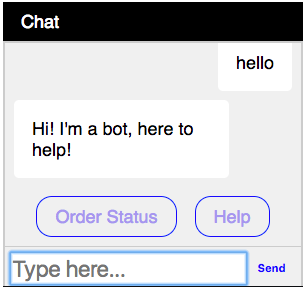
\includegraphics[scale=0.8]{Imagens/chat-exemple.png} 
   \caption{Fonte: Botkit}
  \label{chatweb}
\end{figure}



\section{Integração Com o Slack}

Em 2015 a framework Botkit foi comprada pela Microsoft e alguns serviços foram Migrados para o Microsoft Bot Framework. Essa framework que fica hospedada nos servidores da Microsoft facilita a criação de um único bot que pode ser executado em vários canais de mensagens, incluindo Skype, Group.me, Facebook Messenger, Slack, Telegram, Kik, SMS e e-mail.

Entretanto, para este trabalho soluções hospedadas e pagas não poderiam ser levadas em consideração. Na documentação oficial do Botkit é recomendado que se utilize a framework da Microsoft para integrações com Telegram e outros canais de comunicação.

Devido essa limitação do Botkit não foi possível utilizar o Telegram como canal de comunicação e o Slack foi selecionado. Entretanto, por ser um projeto open source é possível desenvolver um middleware que funcione com o telegram e outros canais em nodejs. 

\subsection{Criando Aplicação na API do Slack}

Para integrar um bot na plataforma do Slack é necessário criar uma conta de desenvolvedor na API oficial\footnote{https://api.slack.com/tutorials}. No Slack, um bot é controlado programaticamente por meio de um token de usuário de bot que tem acesso a uma ou mais APIs do Slack. Além disso, um bot para o slack é uma aplicação que precisa ser criada conforme a figura \ref{cadastro_slack}.

\begin{figure}[H]
  \centering
   \caption{Criando uma aplicação na API do Slack}
  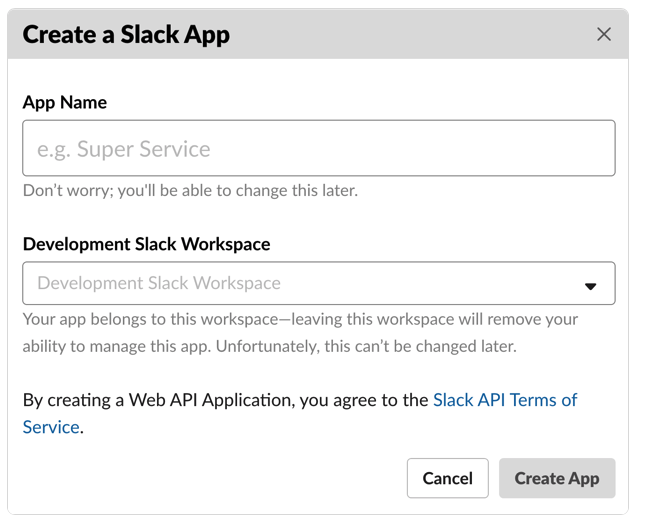
\includegraphics[scale=0.5]{Imagens/slack_cadastro.png} 
  \label{cadastro_slack}
\end{figure}

Assim que a aplicação é criada e autorizada a executar no Slack, as credenciais de seguranças estarão disponíveis. A partir disso, é necessário pegar as credenciais geradas e utiliza-las para inicializar o chatbot como ilustram as figuras \ref{token} e \ref{token_codigo}.

\begin{figure}[H]
  \centering
   \caption{Credenciais de segurançã da API do Slack}
  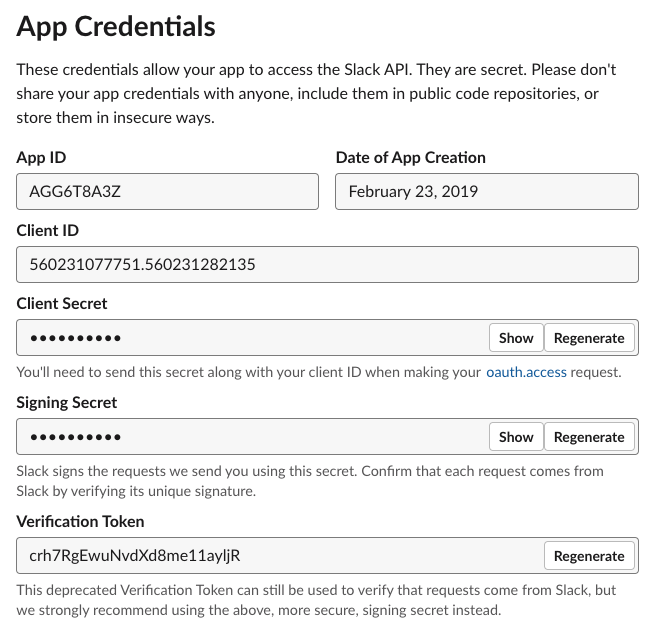
\includegraphics[scale=0.5]{Imagens/slack_token.png} 
  \label{token}
\end{figure}



\begin{figure}[H]
  \centering
   \caption{Código responsável por inicializar o chatbot com as credenciais do Slack}
  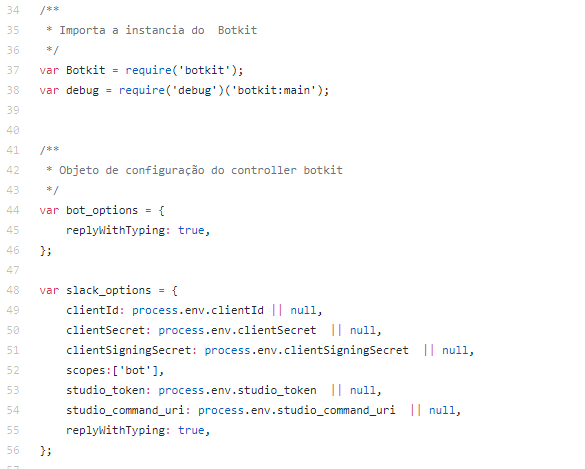
\includegraphics[scale=0.8]{Imagens/config.png} 
  \label{token_codigo}
\end{figure}



\begin{figure}[H]
  \centering
   \caption{Código responsável por inicializar o chatbot com as credenciais do Slack}
  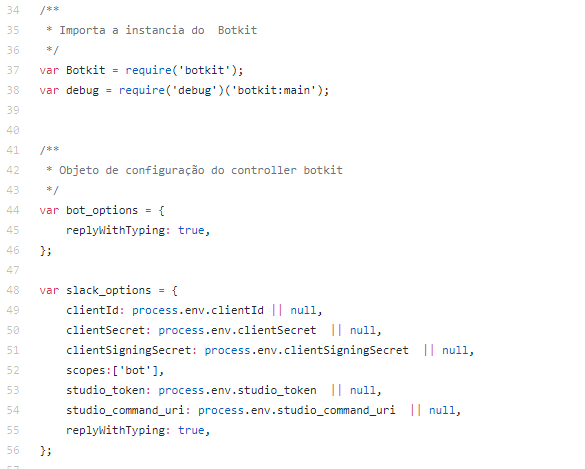
\includegraphics[scale=0.8]{Imagens/config.png} 
  \label{token_codigo}
\end{figure}



Após a obtenção das credenciais que serão usadas para integrar o chatbot no mensageiro configurar a URL do webhook onde serão enviadas as notificações dos eventos. Essa configuração é ilustrada na figura \ref{webhook-slack-config}. Uma vez que essa configuração foi realizada, o slack irá enviar alguns eventos de teste para o servidor webhook que está no endereço fornecido para confirmar o funcionamento da aplicação. Dessa forma, o código responsável por responder os eventos emitidos pelo slack é apresentado na figura X. 


\begin{figure}[H]
  \centering
   \caption{Configuração da URL do webhook.}
  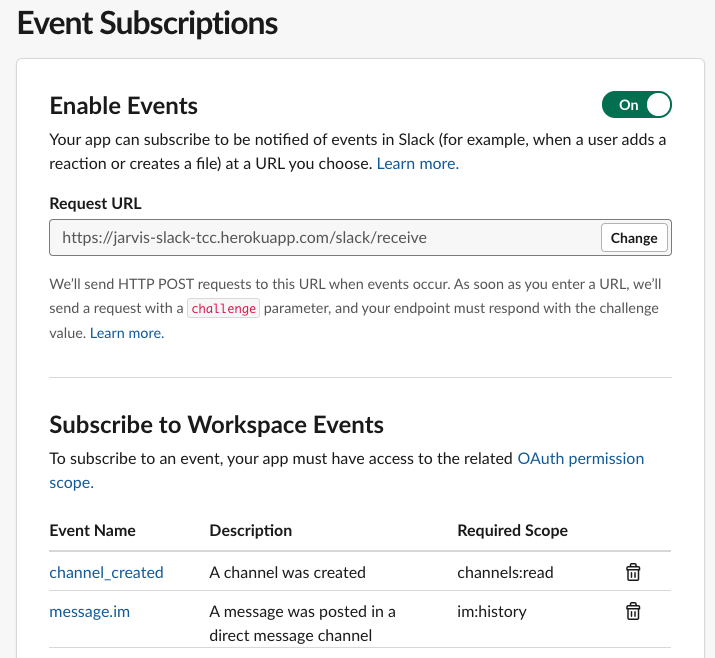
\includegraphics[scale=0.5]{Imagens/Slack_webhook_app.png} 
  \label{webhook-slack-config}
\end{figure}


\begin{figure}[H]
  \centering
   \caption{Código responsável por receber eventos do slack.}
  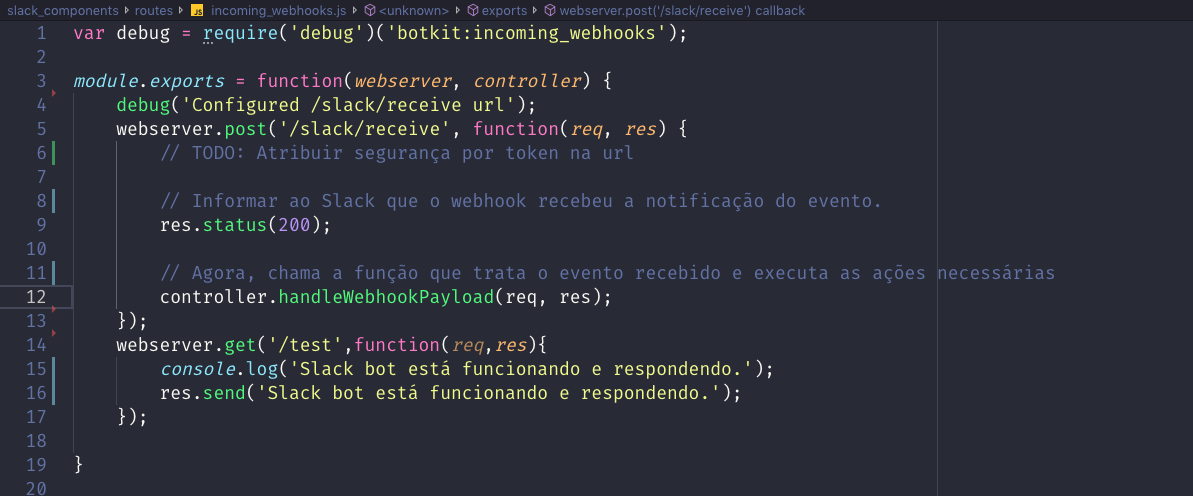
\includegraphics[scale=0.3]{Imagens/webhook-code-slack.png} 
  \label{webhook-slack-config}
\end{figure}




\section{Implantação do Servidor}

Para que o servidor webhook consiga gerenciar as requisições vindas de vários canais, é imprescindível que ele esteja disponível na internet. Sendo assim, para a fase de implantação na web foi utilizado o Heroku\footnote{https://www.heroku.com} e Digital Ocean para hospedar o servidor na nuvem. 

O Heroku é uma plataforma em nuvem como um serviço que suporta várias linguagens de programação. As principais linguagens suportadas são Java, Node.js, Scala, Clojure, Python, PHP e Go. Essa plataforma possui um plano gratuito para desenvolvedores e, portanto, atende as necessidades deste trabalho.

O digital Ocean é um provedor americano de infraestrutura de nuvem com sede em Nova York e data centers em todo o mundo. Sendo assim, foi utilizada uma máquina virtual linux hospedada do digital ocean.

Uma combinação das duas plataformas (Heroku e Digital ocean) foi utilizada pelo fato de que o uso da API do Slack necessita de conexões que utilizam o conexões seguras por meio do protocolo HTTPS. Assim, Após a implantação do código na nuvem, o Heroku disponibiliza uma URL \footnote{Uniform Resource Locator que em português significa "localizador uniforme de recursos". Esse termo se refere ao endereço de rede no qual se encontra algum recurso computacional} que torna público os serviços implementados no servidor webhook e que possui certificado de segurança SSL (\textit{Secure Sockets Layer}) válido. 

Portanto, no servidor digital ocean foi hospedado a maior parte dos serviços que não necessitam de conexão HTTPS e a integração segura com o Slack foi hospedada no Heroku.

O servidor webhook e a interface web do chatbot está disponível na url: \url{https://jarvis-bot-tcc.herokuapp.com}.



\subsection{Integração com Twilio/Whatsapp}

Para que o chatbot fosse capaz de comunicar-se por meio do mensageiro whatsapp foi utilizada a plataforma Twilio. Essa plataforma  quee possibilita que desenvolvedores de software integrem voz, mensagens de texto, video, notificações e facilidades de comunicação em  geral em seus aplicativos. Essa integração pode ser feita usando API ou webhook.

O twilio disponibiliza um ambiente de testes, também chamado de sandbox, onde o desenvolvedor configura uma URL para recebimento de eventos. Dessa forma, quando um usuário envia uma mensagem no whatsapp para um número definido o webhook do twilio dispara esse evento, juntamente com a mensagem, para a URL definida pelo desenvolvedor. O twilio utiliza a API do whatsapp \footnote{https://www.whatsapp.com/business/api}, em inglês Whatsapp Business API, para troca de informações e eventos com o mensageiro.

Vale ressaltar que o facebook, empresa que mantém o whatsapp, limita o uso da API para que somente empresas verificadas tenham acesso. O twilio, portanto, é uma plataforma autorizada e é atualmente o principal meio de comunicação programável com o mensageiro.

Sendo assim, uma conta no twilio foi criada e configurada realizar a integração com o whatsapp. De acordo com a documentação oficial do twilio, é necessário criar um projeto, configurar a URL do webhook e obter as credenciais de acesso como mostras as figuras \ref{twilio-project}, \ref{url-twilio} e \ref{twilio-tokens} respectivamente. 



\begin{figure}[H]
  \centering
   \caption{Criação de um projeto na plataforma twilio.}
  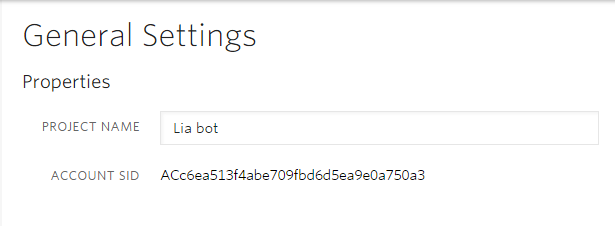
\includegraphics[scale=0.5]{Imagens/twilioproject.PNG} 
  \label{twilio-project}
\end{figure}


\begin{figure}[H]
  \centering
   \caption{Configurando a URL do webhook.}
  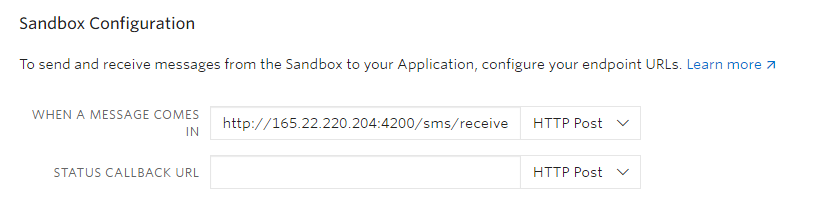
\includegraphics[scale=0.5]{Imagens/urlcallback.PNG} 
  \label{url-twilio}
\end{figure}



\begin{figure}[H]
  \centering
   \caption{Credenciais de acesso geradas pelo twilio.}
  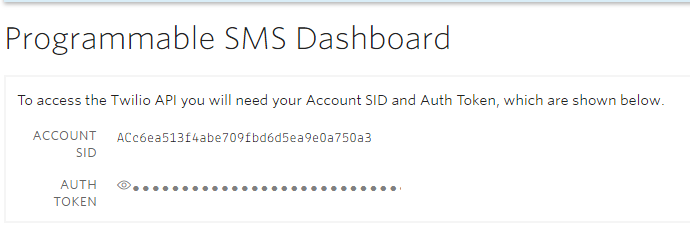
\includegraphics[scale=0.5]{Imagens/tokentwilio.PNG} 
  \label{twilio-tokens}
\end{figure}


Após a configuração da URL como ilutra a figura \ref{url-twilio} foi o webhook foi configurado para atender requisições HTTP nessa URL como mostra as figura \ref{twilio-tokens-code} e \ref{twilio-webhook-code}.


\begin{figure}[H]
  \centering
   \caption{Código responsável por configurar as credenciais de acesso ao twilio.}
  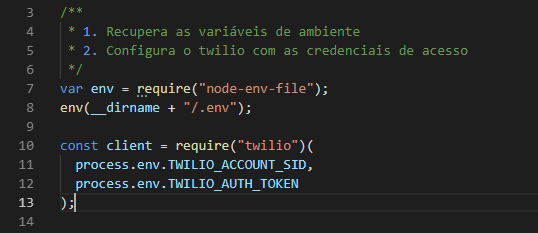
\includegraphics[scale=0.5]{Imagens/twilio-credenciais.PNG} 
  \label{twilio-tokens-code}
\end{figure}


\begin{figure}[H]
  \centering
   \caption{Código responsável por configurar o webhook para receber eventos do twilio}
  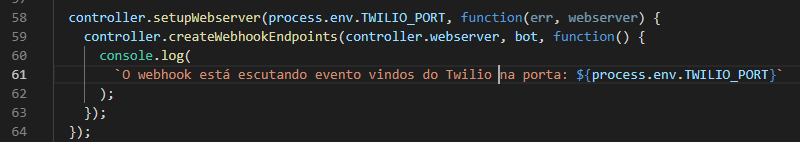
\includegraphics[scale=0.5]{Imagens/twilio-webhook-code.PNG} 
  \label{twilio-webhook-code}
\end{figure}






\chapter{Resultados }

Nesta Seção são apresentados os resultados obtidos com a implantação de um ambiente de trabalho para o funcionamento do chatbot em uma pagina web, slack e whatsapp. A integração permitiu que o chatbot, chamado de lia, pudesse estar presente em todos os canais propostos e exemplos de conversas nesses canais são ilustrados.

\section{Conversa com o chatbot no Slack}

O slack é uma plataforma de comunicação principalmente para empresas, abrangente e com funcionalidades que lembram um chat que também faz chamadas em vídeo, só que com muito mais capacidade de customização e interação entre os participantes, além de comandos ágeis e facilidade para compartilhar os mais diversos tipos de arquivos. Nesse mensageiro é possível:


\begin{itemize}
    \item Criar times: Um time normalmente será por onde você gerenciará a comunicação interna de sua empresa, por exemplo. É possível criar mais de um time caso sua empresa seja dividida em unidades de negócios, como diretoria de marketing e vendas.

    \item Criar canais: Para cada time você cria canais com seus assuntos de interesse. Por exemplo: criação, atendimento ao cliente, produção, desenvolvimento, suporte etc. Esses canais podem ser públicos, com acesso de todos os participantes da empresa, ou fechados.

    \item Enviar Mensagens diretas: Quer falar diretamente com alguém? Você pode trocar mensagens diretamente com uma pessoa ou grupo sem que o canal inteiro participe e não precisa recorrer ao WhatsApp.

    \item Executar Comandos Slash: O Slack tem uma série de comandos para facilitar sua vida. Por exemplo, se quer citar uma pessoa, use '@nomedapessoa', ou se quer notificar um canal, use '#nomedocanal', quando estiver digitando sua mensagem.
\end{itemize}

Portanto, uma vez realizada a integração com o slack o chatbot pode se comunicar por meio de times, canais, mensagens diretas e outros comandas existentes.  As figuras \ref{slack01} e \ref{slack02} mostram uma conversa com o chatbot por meio de mensagens diretas e a figura \ref{slack03} mostra o chatbot respondendo a uma citação.


\begin{figure}[H]
  \centering
   \caption{Mensagem direta com o chatbot no slack.}
  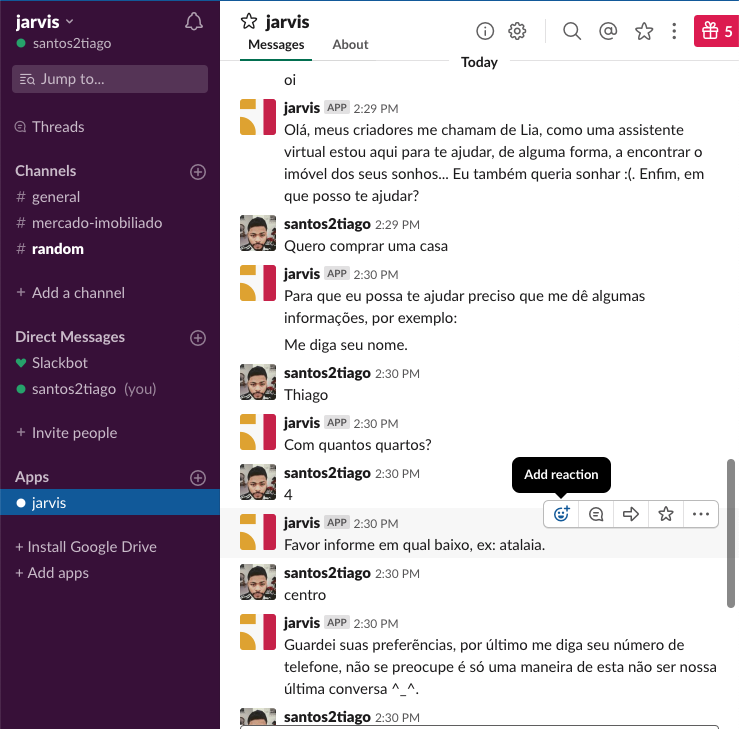
\includegraphics[scale=0.5]{Imagens/slack01.png} 
  \label{slack01}
\end{figure}


\begin{figure}[H]
  \centering
   \caption{Mensagem direta com o chatbot no slack.}
  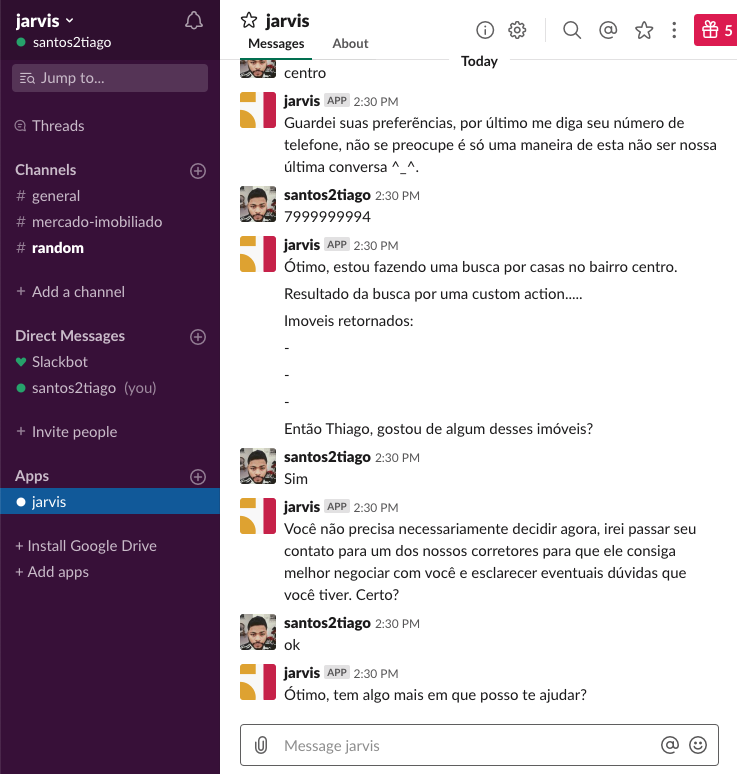
\includegraphics[scale=0.5]{Imagens/slack02.png} 
  \label{slack02}
\end{figure}



\begin{figure}[H]
  \centering
   \caption{Conversa com o chatbot por citação no slack.}
  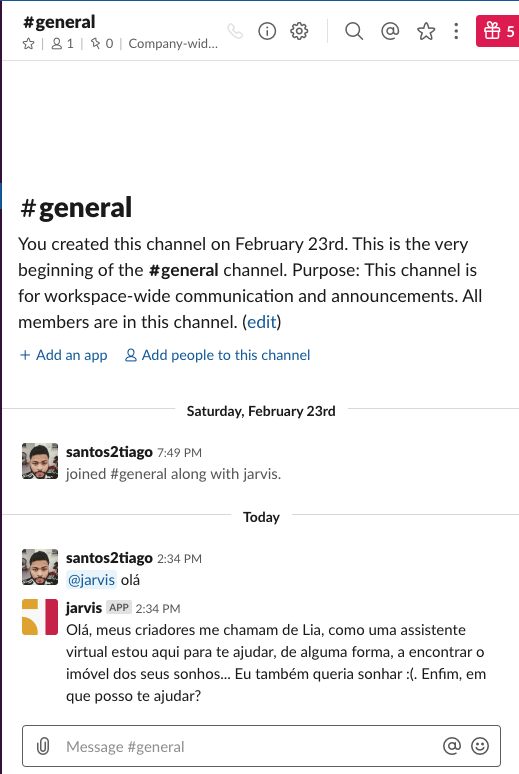
\includegraphics[scale=0.5]{Imagens/slack03.png} 
  \label{slack03}
\end{figure}

\section{Conversa com o chatbot na Web}

Para iniciar uma conversa com o chatbot na web basta acessar a URL a seguir:

\begin{itemize}
    \item http//165.22.220.204:8443/chat.html
\end{itemize}


\begin{figure}[H]
  \centering
   \caption{Iniciando conversa com o chatbot na web.}
  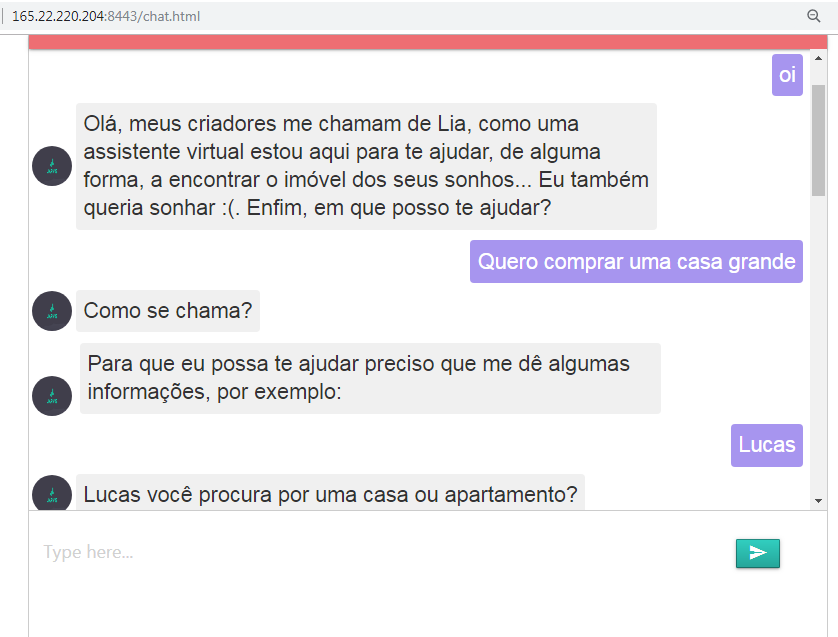
\includegraphics[scale=0.5]{Imagens/chat1.PNG} 
  \label{twilio-webhook-code}
\end{figure}

\begin{figure}[H]
  \centering
   \caption{conversa com o chatbot.}
  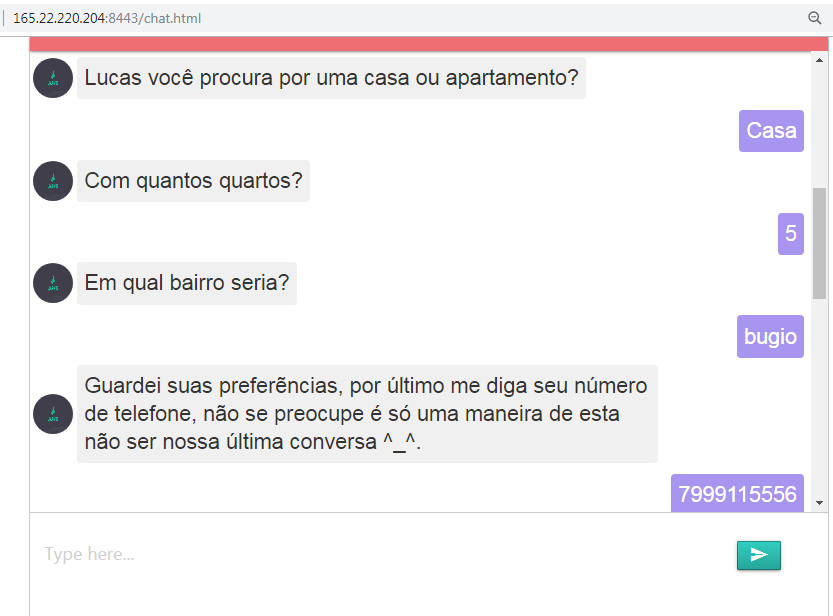
\includegraphics[scale=0.5]{Imagens/chat2.PNG} 
  \label{twilio-webhook-code}
\end{figure}

\begin{figure}[H]
  \centering
   \caption{conversa com o chatbot.}
  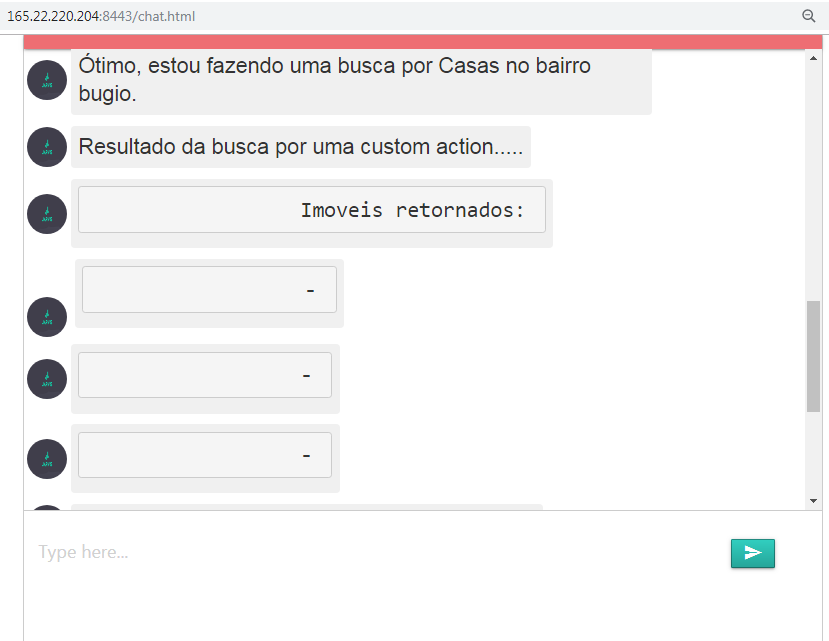
\includegraphics[scale=0.5]{Imagens/chat3.PNG} 
  \label{twilio-webhook-code}
\end{figure}



\section{Conversa com o chatbot no Whatsapp}

O ambiente de desenvolvimento do twilio, chamado de sandbox, possui três números de telefone pré-configurados como contas comerciais do whatsapp e são compartilhados entre todos os usuários do sandbox. Para usar o Sandbox, você deve começar optando pelo sandbox enviando o número de telefone que escolheu uma mensagem do WhatsApp. Uma vez ativado, você receberá apenas mensagens da sua Sandbox específica. A configuração da sendbox para este trabalho está ilustrada na figura \ref{twilio-sandbox}.


\begin{figure}[H]
  \centering
   \caption{Configurando o sandbox do twilio entrar no canal de comunicação do chatbot.}
  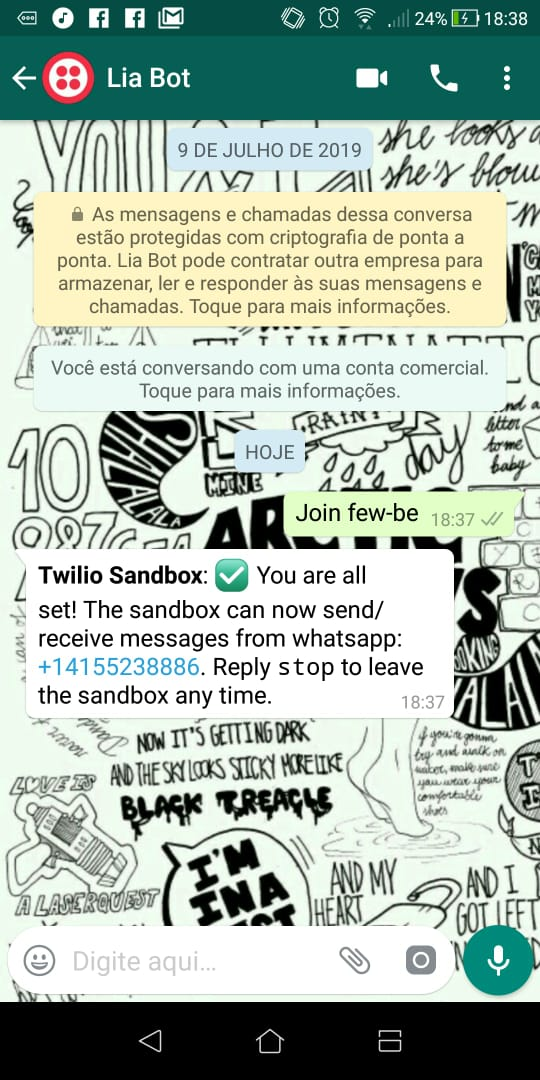
\includegraphics[scale=0.35]{Imagens/twilio-sandbox.jpeg} 
  \label{twilio-sandbox}
\end{figure}


Uma vez configurado o ambiente de desenvolvimento, o sandbox, é possível conversar normalmente com o chatbot. As figura \ref{twilio-conversa1}, \ref{twilio-conversa2}, e \ref{twilio-conversa3} mostram um exemplo de diálogo.


\begin{figure}[H]
  \centering
   \caption{Conversando com o chatbot no whatsapp.}
  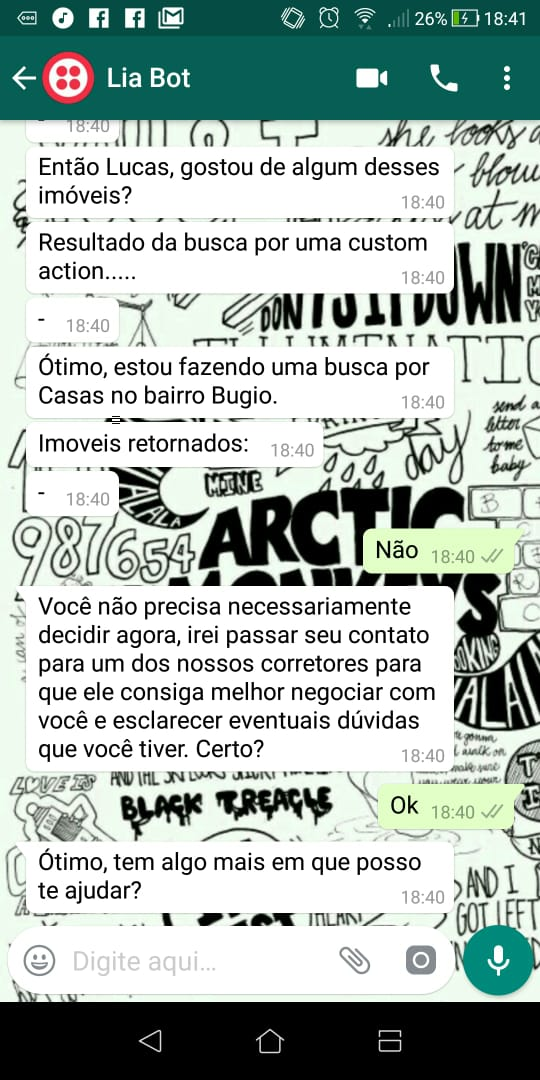
\includegraphics[scale=0.5]{Imagens/twilio-conversa1.jpeg} 
  \label{twilio-conversa1}
\end{figure}

\begin{figure}[H]
  \centering
   \caption{Conversando com o chatbot no whatsapp}
  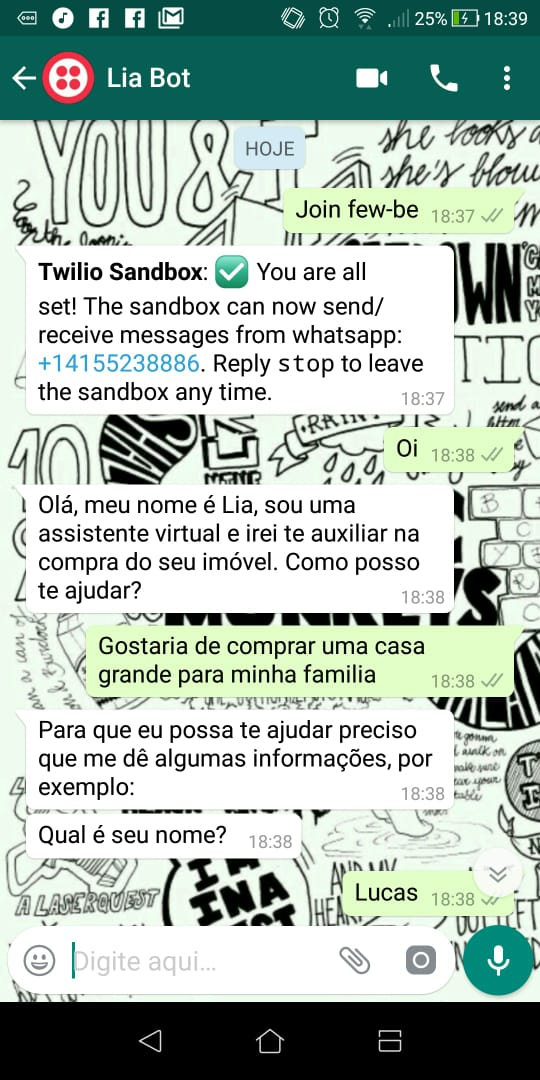
\includegraphics[scale=0.5]{Imagens/twilio-conversa2.jpeg} 
  \label{twilio-conversa2}
\end{figure}


\subsection{Extensão da integração}

A partir da definição da arquitetura modular e com partes que possuem funções coesas foi possível realizar a extensão da integração em mais um canal, o Whatsapp. Assim, uma vez que a base de conhecimento ou cérebro do chatbot está em funcionamento de acordo com a arquitetura é possível, com algumas modificações no conector, realizar a integração em outros canais. 

Vale destacar que a proposta de integração deste trabalho é flexível e não necessariamente precisa ser adotada para o desenvolvimento de chatbots. Entretanto, a arquitetura modularizada e coesa, um artefato gerado neste trabalho, deve ser adotada para evitar um alto acoplamento que pode causar problemas para evoluir o software.

De maneira geral, para adição de novos canais é necessário o entendimento da arquitetura e configuração de uma nova URL para o webhook do servidor no canal pretendido.


\subsection{Validação}

A validação do chatbot foi realizada em duas etapas. Em um primeiro momento foi feito um teste automatizado do servidor webhook, sendo que foi utilizada uma ferramenta que realiza testes por meio de requisições HTTP e exibe os resultados obtidos bem como o sucesso o falha do teste. Após essa primeira validação, o chatbot foi submetido a testes de estresse também com o uso de uma ferramenta de automatização de testes.


\subsubsection{Tarefa um de validação}
Neste passo foi utilizada a ferramenta online API TESTER\footnote{https://apitester.com/} onde é possível Fazer solicitações HTTP, extrair valores das respostas, verificar que os valores estão corretos, separar os testes por etapas, reutilizar variáveis nas etapas ou criar lógica customizada usando JavaScript. Portanto, um teste com quatro passos foi construído para validar e verificar que o servidor webhook está funcionando e respondendo adequadamente as mensagens dos usuários.

Com essa ferramenta é possível criar um teste com vários passos e, portanto, o teste criado foi dividido em quatro passos e tem o objetivo exclusivo de  verificar se a integração foi bem sucedida e está respondendo e atendendo as requisições dos usuários. Esse teste não tem o objetivo de cobrir todas as possibilidades de conversas entre o chatbot e o usuário mas verificar se a integração está funcional. Ou seja, o teste tem o intuito de verificar se para casa mensagem enviada no lado cliente existe uma resposta do chatbot.


\begin{figure}[H]
  \centering
   \caption{Passo um: Verifica se o servidor está online e funcionando.}
  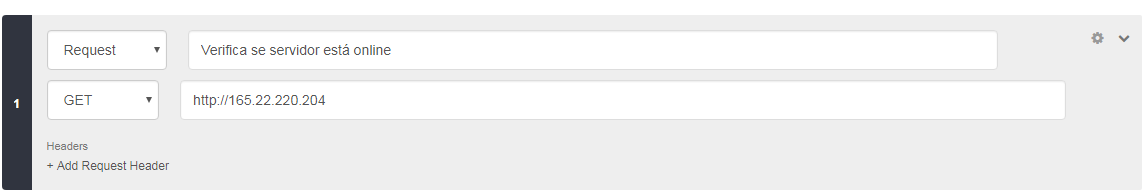
\includegraphics[scale=0.5]{Imagens/passo1.PNG} 
  \label{teste1}
\end{figure}

\begin{figure}[H]
  \centering
   \caption{Passo dois: Simula um usuário cumprimentando o chatbot.}
  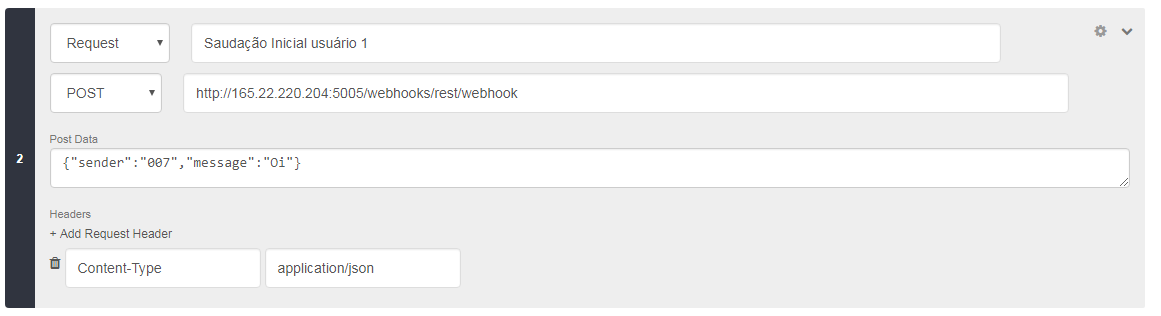
\includegraphics[scale=0.5]{Imagens/passo2.PNG} 
  \label{teste2}
\end{figure}

\begin{figure}[H]
  \centering
   \caption{Passo três: Simula outro usuário cumprimentando o chatbot.}
  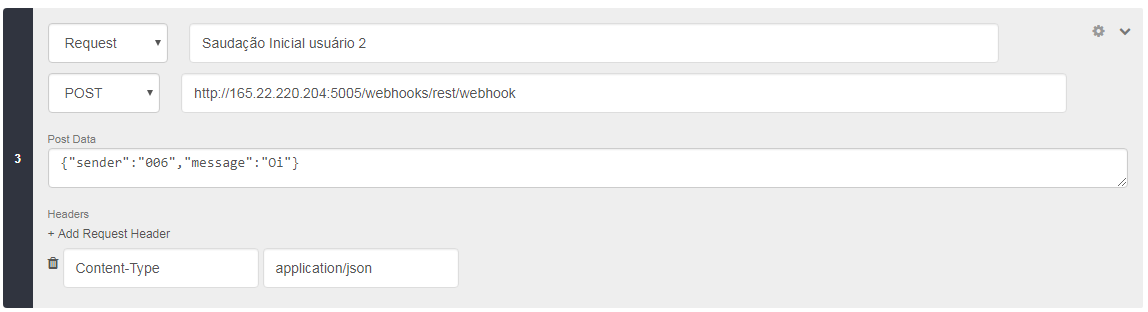
\includegraphics[scale=0.5]{Imagens/passo3.PNG} 
  \label{teste3}
\end{figure}

\begin{figure}[H]
  \centering
   \caption{Passo quatro: Simula um usuário com intençao de comprar um imóvel.}
  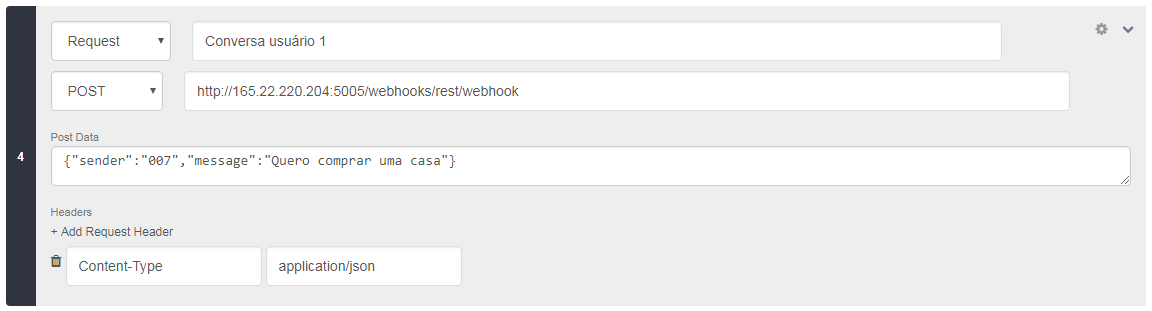
\includegraphics[scale=0.5]{Imagens/passo4.PNG} 
  \label{teste4}
\end{figure}

Após a execução do teste verificou-se que todos quatro passos obtiveram sucesso e a integração foi bem sucedida. as figuras \ref{resultado-teste1}, \ref{resultado-teste2}, \ref{resultado-teste3} e \ref{resultado-teste4} mostram o resultado obtido após a execução do teste.

\begin{figure}[H]
  \centering
   \caption{Resultado do passo um.}
  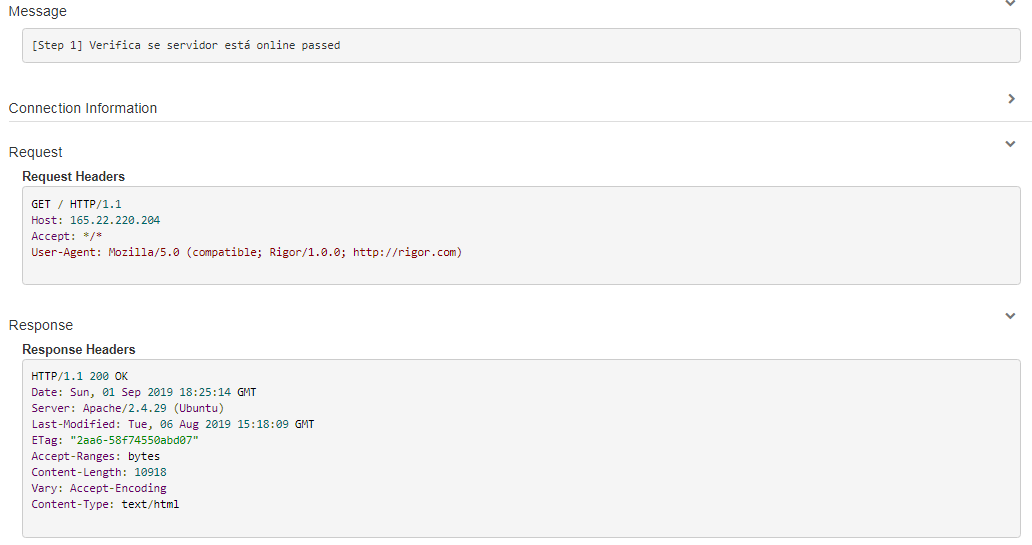
\includegraphics[scale=0.5]{Imagens/resultado1.PNG} 
  \label{resultado-teste1}
\end{figure}


\begin{figure}[H]
  \centering
   \caption{Resultado do passo dois.}
  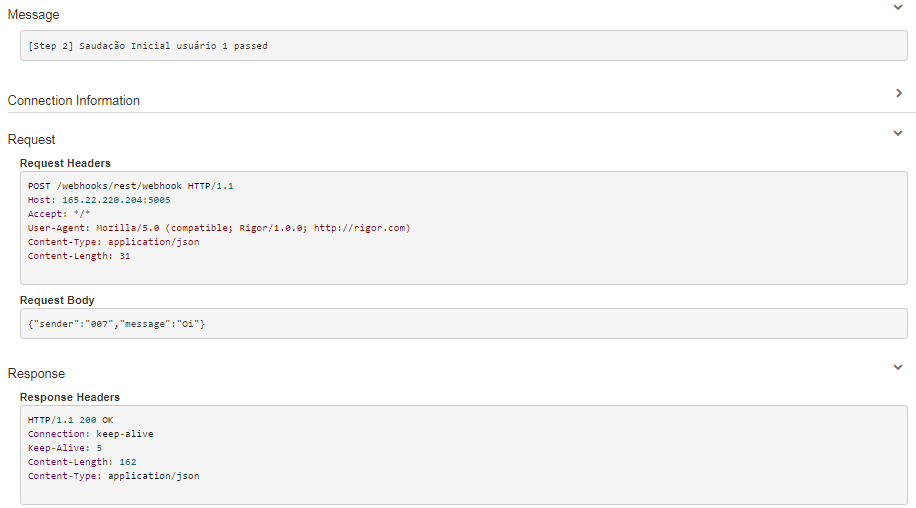
\includegraphics[scale=0.5]{Imagens/resultado2.PNG} 
  \label{resultado-teste2}
\end{figure}


\begin{figure}[H]
  \centering
   \caption{Resultado do passo três.}
  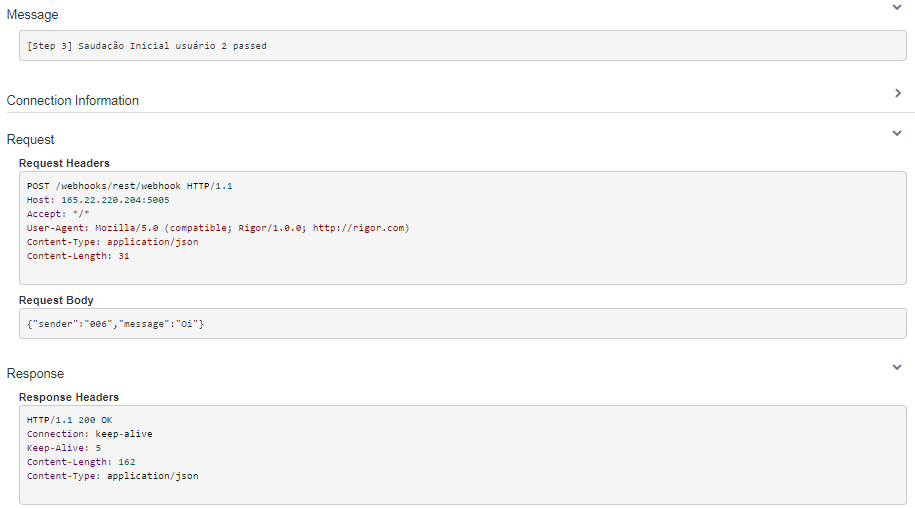
\includegraphics[scale=0.5]{Imagens/resutado3.PNG} 
  \label{resultado-teste3}
\end{figure}


\begin{figure}[H]
  \centering
   \caption{Resultado do passo quatro.}
  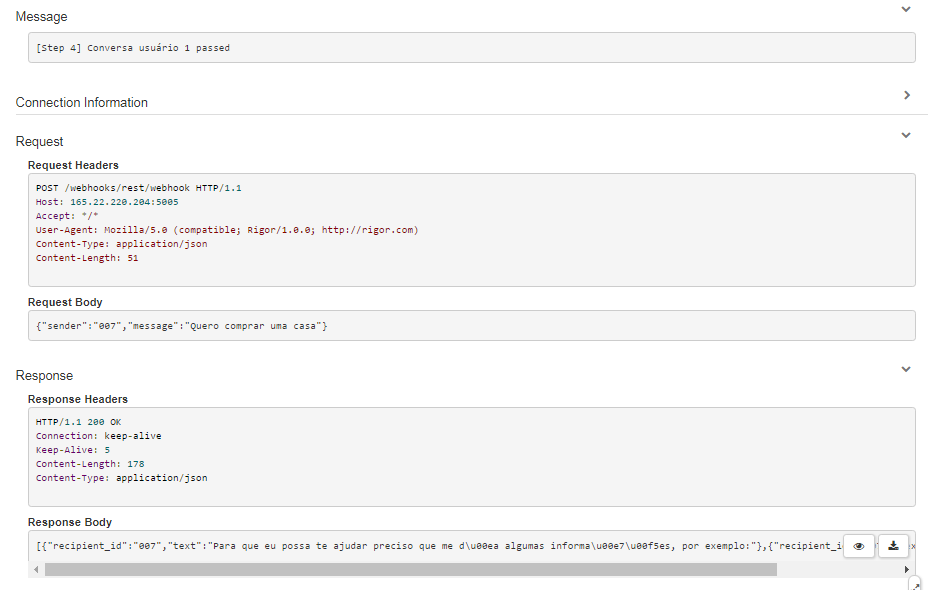
\includegraphics[scale=0.5]{Imagens/resultado4.PNG} 
  \label{resultado-teste4}
\end{figure}


\subsubsection{Tarefa dois de validação}
Neste passo foi utilizada a ferramenta online RESTFUL STRESS\footnote{https://chrome.google.com/webstore/detail/restful-stress/lljgneahfmgjmpglpbhmkangancgdgeb} onde é possível realizar testes de estresse por meio do protocolo HTTP e verificar que os valores estão corretos de acordo com o número de requisições definidas. A ferramenta disponibiliza gráficos com os resultados dos testes.

Um teste de estresse é realizado para submeter o software a situações extremas. Basicamente, o teste de estresse baseia-se em testar os limites do software e avaliar seu comportamento. Assim, avalia-se até quando o software pode ser exigido e quais as falhas, se existirem, decorrentes do teste. As figuras X,Y e Z mostram que os resultados obtidos.


\begin{figure}[H]
  \centering
   \caption{Resultado de teste de estresse para 10 requisições}
  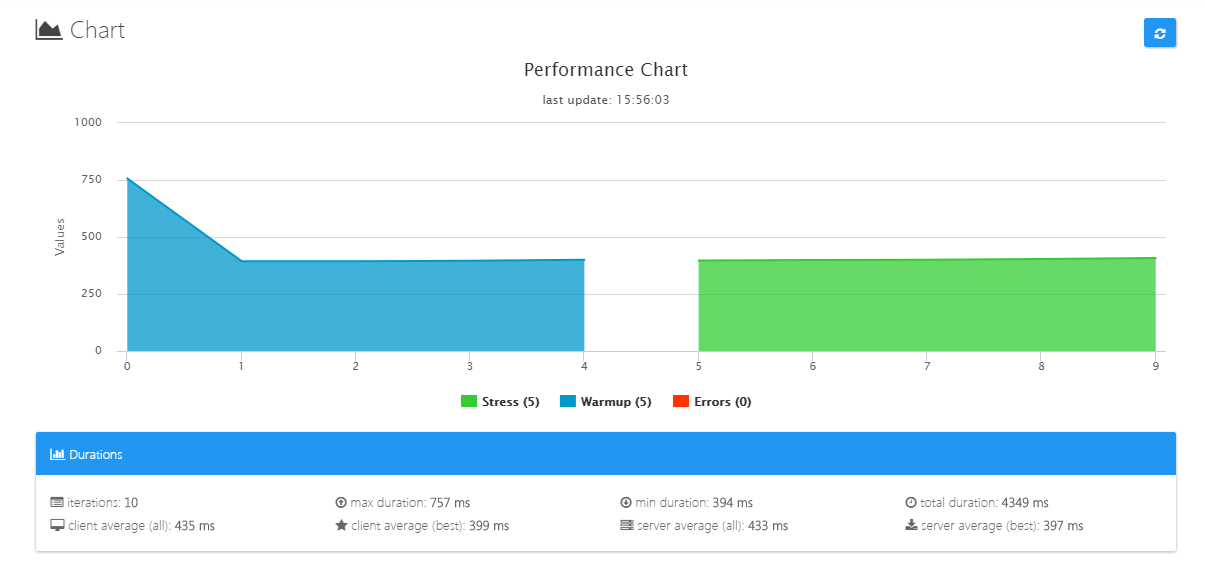
\includegraphics[scale=0.5]{Imagens/estresse10.PNG} 
  \label{estresse1}
\end{figure}

\begin{figure}[H]
  \centering
   \caption{Resultado de teste de estresse para 100 requisições.}
  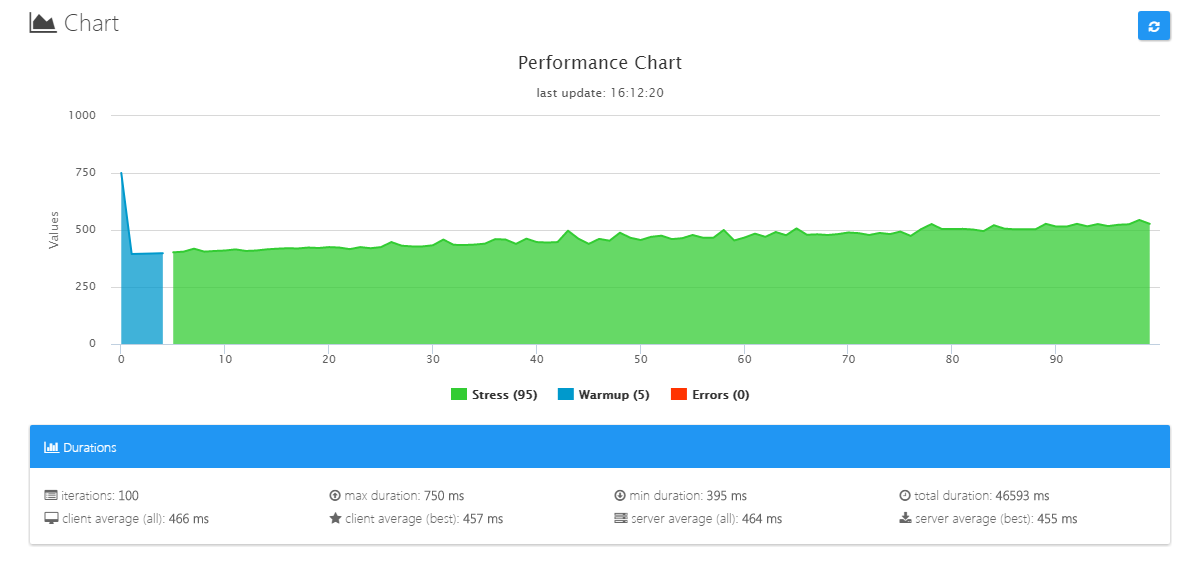
\includegraphics[scale=0.5]{Imagens/estrese100.PNG} 
  \label{estresse2}
\end{figure}

\begin{figure}[H]
  \centering
   \caption{Resultado de teste de estresse para 10 mil requisições.}
  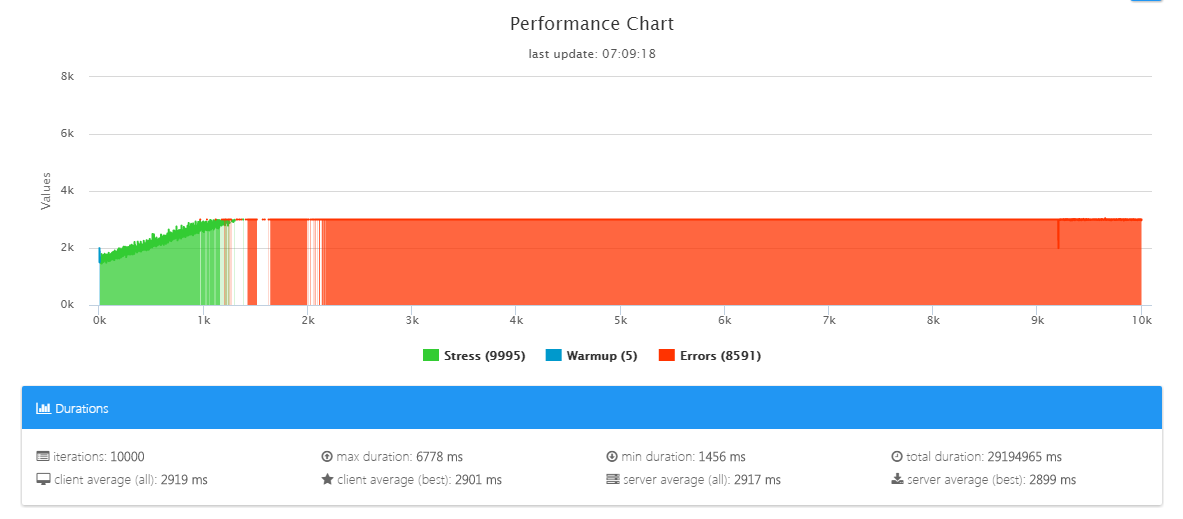
\includegraphics[scale=0.5]{Imagens/perfomance10k.PNG} 
  \label{estresse3}
\end{figure}


Para realização deste teste foi utilizada uma instância do servidor webhook executando em uma maquina virtual com as seguintes configurações:

\begin{itemize}
    \item 1GB de memória ram
    \item 25GB de disco
    \item Sistema operacional linux ubuntu 18.04 (LTS) x64 
\end{itemize}


Após a realização da tarefa dois ficou evidente que a integração de chatbots deve também levar em consideração os aspectos relacionados a escalabilidade. Ou seja, refletir sobre a hipótese do uso do software pelo usuário finais crescer e o sistema não conseguir atender as demandas. Vale ressaltar que a escalabilidade da aplicação não é um problema de integração mas de infraestrutura. Uma solução comum para realizar o gerenciamento de concorrência é realizar balanceamento de carga por meio de clusters\footnote{o termo cluster faz referência à arquitetura de sistema que une dois ou mais computadores ou aplicações como se fossem apenas um.} que possuem várias instâncias da aplicação executando. Esse é um problema que é sanado ao utilizar plataformas como Watson que possuem uma infraestrutura como serviço para os clientes.


\chapter{Conclusões}

Com o avanço dos estudos na área de Inteligência
Artificial, os chatbots estão cada vez mais presentes e popularizados, sendo em
forma de serviço de Atendimento ao consumidor, em forma de comunicação e marketing ou até em formas mais
avançadas.


O presente trabalho visou a integração de um chatbot em pelo menos dois canais como estudo de caso para conversar e responder as perguntas de clientes interessados no mercado imobiliário, ou seja, compra e venda de imóveis. Uma das vantagens na utilização de chatbots em mais de um canal de comunicação é alta disponibilidade do serviço nos canais de preferência dos usuários finais. Além do mais, o curto tempo de resposta e a capacidade de interagir com milhões de usuários simultaneamente fazem dos chatbots uma ferramenta de grande utilidade comercial. 

Após o desenvolvimento do chatbot pode-se concluir, a partir da primeira tarefa de validação, que ele conseguiu responder e interagir em um nível em todos os canais propostos, que foram uma pagina web e o mensageiro slack, além do whatsapp que foi um canal adicional. Com a integração realizada nos canais de comunicação um chatbot pode, portanto, interagir com usuários em qualquer horário e com capacidade de manter um diálogo simultâneo com diversas pessoas.

Paralelamente, a tarefa de validação dois, que consistiu em testes de estresse, submeteu o chatbot a situações em que ocorreria milhares de requisições simultâneas para testar situações em que os limites do software estariam em extremo e avaliar seu comportamento. Neste ponto a integração do chatbot respondeu e se comportou adequadamente como esperado.

A integração foi implementada por meio das frameworks de desenvolvimento de código aberto Rasa e Bokit. Sendo assim, esse estudo verificou que é possível optar por uma alternativa de código aberto e grátis obtendo eficiência na integração em escala em oposição as soluções proprietárias e pagas. Entretanto, não existe bala de prata no desenvolvimento de software e o uso das frameworks adotadas neste trabalho não deve ser considerado uma regra.

Também ficou comprovado que uma vez que a base de conhecimento ou cérebro do chatbot está em funcionamento de acordo com a arquitetura é possível, com algumas modificações no conector, realizar a integração em outros canais. Destacando-se que a proposta de integração deste trabalho é flexível e não necessariamente precisa ser adotada para o desenvolvimento de chatbots. Entretanto, a arquitetura modularizada e coesa, um artefato gerado neste trabalho, deve ser adotada para evitar um alto acoplamento que pode causar problemas para evoluir o software. 



Para trabalhos futuros é necessário o desenvolvimento de adaptadores de código aberto que consiga realizar a comunicação do chatbot em mais canais de comunicação. Além disso, criar uma interface visual para que usuários não técnicos possam distribuir o chatbot nos canais disponíveis. 



\bibliography{Bibliografia}

% ----------------------------------------------------------
% ELEMENTOS PÓS-TEXTUAIS
% ----------------------------------------------------------
\postextual

\renewcommand{\chapnumfont}{\chaptitlefont}
\renewcommand{\afterchapternum}{}


% ----------------------------------------------------------
% 
%    \begin{apendicesenv}

% Imprime uma página indicando o início dos apêndices
\partapendices

% ----------------------------------------------------------
\chapter{Quisque libero justo}
% ----------------------------------------------------------

\lipsum[50]

% ----------------------------------------------------------
\chapter{Nullam elementum urna vel imperdiet sodales elit ipsum pharetra ligula
ac pretium ante justo a nulla curabitur tristique arcu eu metus}
% ----------------------------------------------------------
\lipsum[55-57]

\end{apendicesenv}

%    \begin{anexosenv}


% Imprime uma página indicando o início dos anexos
\partanexos

% ---
\chapter{Morbi ultrices rutrum lorem.}
% ---
\lipsum[30]

% ---
\chapter{Cras non urna sed feugiat cum sociis natoque penatibus et magnis dis
parturient montes nascetur ridiculus mus}
% ---

\lipsum[31]

% ---
\chapter{Fusce facilisis lacinia dui}
% ---

\lipsum[32]


\end{anexosenv}

% ----------------------------------------------------------

\end{document}